\documentclass[11pt,a4paper]{book}
\usepackage{amsmath}
\usepackage[english]{babel}
\usepackage{graphicx}
\usepackage{picture}
\usepackage{color}
\usepackage{graphpap,color}
\usepackage{subfig}
\usepackage[percent]{overpic}

\usepackage[english]{babel}
\usepackage{amsfonts}
\usepackage{amssymb}
\usepackage{makeidx}
\usepackage[Lenny]{fncychap} %Sonny, Lenny, Glenn, Conny, Rejne, Bjarne, Bjornstrup
\usepackage{pdflscape}
%\usepackage{booktabs}
%\usepackage[usenames,dvipsnames,svgnames,table]{xcolor}
\definecolor{kuleuven}{RGB}{29,141,176}
\definecolor{kuleuven1}{RGB}{82,189,236}
\usepackage[]{geometry} %bindingoffset=25mm  hmarginratio=2:3
\usepackage{hyperref}
\usepackage{mathrsfs}
%\usepackage{layout} \layout

\newcommand{\nocontentsline}[3]{}
\newcommand{\tocless}[2]{\bgroup\let\addcontentsline=\nocontentsline#1{#2}\egroup}

\makeindex
\begin{document}
%\renewcommand*\chaptername{Hoofdstuk}
%\renewcommand*\bibname{Bibliografie}
%\renewcommand*\appendixname{Bijlagen}

\frontmatter
\newgeometry{textwidth=540pt,textheight=780pt,top=20pt,left=20pt,right=20pt}
\begin{titlepage}

\begin{figure}[tc]{%
      \begin{overpic}[width=1\textwidth,natwidth=50,natheight=0]{img/Picture1.png}
        \put(35,4){\color{white}{\textbf{FACULTEIT ECONOMIE EN BEDRIJFSWETENSCHAPPEN}}}
      \end{overpic}
    }
\end{figure}

\vspace*{4.5cm}
{\color{kuleuven1}{\Huge Identification of important contributions}}

{\color{kuleuven1}{\Huge in diagnostic medical imaging}}

\vspace*{0.5cm}
{\Large Identificatie van belangrijke contributies in diagnostische medische beeldvorming}

\begin{figure}[bl]
  %\centering
   \begin{minipage}[c]{0.4\textwidth}  {%
      \begin{overpic}[width=0.9\textwidth,natwidth=300,natheight=370]{img/Picture2.png}
        \put(70,45){\begin{minipage}[c]{1.80\textwidth}
\begin{flushright}

{\Large Ir. Sven Van Hove} \linebreak
{s0190440} \linebreak
   
\textbf{{\large Masterproef aangeboden tot  \linebreak
het behalen van de graad}} \linebreak
\linebreak
{\large \textsc{Master in het Management}}\linebreak
{\large }\linebreak
\linebreak
\textbf{{\large Promotor:}}  Prof. Dr. R. Veugelers \linebreak
\textbf{{\large Werkleider:}} D. Verhoeven
\linebreak

\textbf{{\large Academiejaar}} {\large 2013-2014}
\linebreak
\end{flushright}
  \end{minipage}}
      \end{overpic}
    }
  \end{minipage}
  
  
\begin{picture}(540,0.2)
\put(0,0){\colorbox{kuleuven1}{\makebox(540,0.2){}}}
\end{picture}
\end{figure}

\end{titlepage}
%%%%%%%%%%%%%%%%%%%%%%%%%%%%%%%%%%%%%%%%%%%%%%%%%%%%%%%%%%%%%%%%%%%%%%%%%%%%%%%%%%%%%%%%%%%%%%%%%%%%
\restoregeometry
\setcounter{equation}{1}

\pagestyle{empty}

%\chapter*{Abstract\hfill}\addcontentsline{toc}{chapter}{Abstract}

\cleardoublepage
\thispagestyle{plain}
\begin{center}
    \Huge 
    Identification of important contributions in diagnostic medical imaging
    
    \vspace{0.5cm}
    
    \large
    Identificatie van belangrijke contributies in diagnostische medische beeldvorming
    
    \vspace{1.0cm}
    
    Sven Van Hove, Dennis Verhoeven, Reinhilde Veugelers
    
    \vspace{0.5cm}
    
	Managerial Economics, Strategy and Innovation (MSI)\\
	Faculteit Economie en Bedrijfswetenschappen\\
	KU Leuven
    
    \vspace{1.0cm}
    \textbf{Abstract}
\end{center}

Radical innovations have the power to disrupt whole technological fields, and
are often seen as a key factor in long term growth. Therefore it is critical to
identify early on how radical an innovation is. In this thesis, we performed a
manual assessment of five interesting innovations in the field of diagnostic medical
imaging: digital radiography, electron beam computed tomography, magnetic
resonance imaging, 18F-FDG tracers in nuclear medicine and the application of
computer aided detection and diagnosis in mammography. The assessment was
performed based on a framework proposed by \cite{verhoeven}. This framework
contains three dimensions: novelty of knowledge origins, novelty of
functionality  and technological impact. The resulting scores turned out lower
than expected, so we looked into possible causes. In the future these scores can
be compared against the outcome of an automatic assessment based on patent
indicators. Conclusions drawn from this comparison could be used to optimize the
framework.

\vspace{1.0cm}

\textbf{Keywords:} important technological inventions, radical innovation,
diagnostic medical imaging, manual assessment, patent indicators.

\tableofcontents

%%%%%%%%%%%%%%%%%%%%%%%%%%%%%%%%%%%%%%%%%%%%%%%%%%%%%%%%%%%%%%%%%%%%%%%%%%%%%%%%%%%%%%%%%%%%%%%%%%%%%%%%%

\setlength{\parindent}{0cm}
\setlength{\parskip}{2ex plus 1ex minus 1ex}

\mainmatter
\pagestyle{headings}

\chapter{Introduction}\label{chap:intro}
\section{Identification of important contributions in a technological field or industry}
In the search for value creation on both the micro- and the macroeconomic scale,
technological innovation has long been considered a very important factor. Some
would argue that it is a key factor in long term growth \cite{arts}. This
innovation comes in many forms, from a simple evolution of the previous state of
the art to a veritable revolution that causes a paradigm shift. To that end, a
lot of research has already been done to clarify what such a revolution or
radical innovation is, and how we can quantify it \cite{structure, invention,
verhoeven}. With this information, researchers hope to one day predict with
high accuracy how much of a breakthrough an idea will be, even before it enters
the market.

\subsection{Innovation framework}
In this text, we will work with the framework proposed by \cite{verhoeven}.
This article proposes both technological and economical dimensions on which to
rank innovation. We will focus on the three technological dimensions: new
knowledge origins, new functionality and impact. Each of these will be explained
in the following paragraphs.

\subsubsection{Novelty in knowledge origins}
The first two dimensions look at the underlying technology of an invention. In
particular, the first dimension is concerned with the knowledge origins. For an
innovation to work as intended, a number of problems usually have to be solved
first. The various sources of knowledge used to solve these problems are
appropriately called knowledge origins. Non-disruptive innovations typically
draw from the same knowledge origins compared to related technologies. On the
other hand, radical innovations often use knowledge from an entirely different
origin. Furthermore, we can distinguish scientific from technological origins.

\subsubsection{Novelty in functionality}
Besides knowledge origins, novelty in functionality is another dimension based
on the underlying technology. That is, radical inventions often use 
new (combinations of) components and principles compared to previous related
innovations.

\subsubsection{Impact}
The third dimension proposed is impact on future technological development.
While technology mostly evolves along a relatively straightforward path,
disruptive innovations often offer a whole new way of thinking - a paradigm
shift. If successful, future innovations are likely to continue down that new
path. In other words, the more the innovation under scrutiny impacts future
developments, the more likely it is to be a radical innovation. Impact can be
direct or indirect, and can be very broad (i.e., affecting other fields than
its own).

\subsubsection{Assessment methodology}
To perform a manual assessment of a certain innovation, some standard questions
related to these three dimensions need to be answered with a score. Those
scores should be substantiated by the relevant literature  or - if possible - by
an expert in the field. The complete assessment sheet can be found in
\autoref{app:score}.

\subsection{Patent indicators}
The framework not only defines the relevant dimensions and manual assessment
methods, but also proposes similar patent indicators. Patents provide a rich
source of data because they not only refer to the inventing entity, but also
offer plenty of forward and backward citations that can be analysed. These allow
us to find the true origin of a new technique, and estimate the impact a patent
had on future research. On top of that, advanced computer algorithms can use
them as a source for data mining and big data techniques. This allows us to
automate part of the process, and gain new insights at the same time. One
limitation of the patent database we work with, is that it only contains
reliable data from 1980 onwards. Because of this, we will constrain ourselves to
assessing inventions in that specific time span.

\section{Goal of this thesis}
In this thesis we will perform a manual assessment of a certain technological
field based on the framework explained above. The field of choice is diagnostic
medical imaging. This was chosen because it sits nicely on the intersection
between biomedical engineering and computer science, two domains the author is
fairly familiar with.

Before we can dive into that, \autoref{chap:imaging} introduces us to
diagnostic medical imaging. Various imaging modalities, such as CT and MRI
scanners will be discussed at length. Once we have a basic understanding of the
most important techniques, \autoref{chap:inventions} will guide us through the
actual assessment of some interesting breakthroughs in the field.

Future research will compare the results of this thesis with the outcome of an
automated assessment based on patent indicators. This will provide the required
feedback for and validation of the proposed framework and patent indicators.

% \subsection{Structure of this text}
% In this chapter, we properly defined our framework of radical innovation.
% Next, \autoref{chap:imaging} introduces us to diagnostic medical imaging, our
% technological field of choice. Various imaging modalities, such as CT and MRI
% scanners will be discussed at length. As soon as we have a basic understanding
% of this field, \autoref{chap:inventions} will highlight some of the most
% interesting breakthroughs since 1980. These breakthrough will be analysed using
% the aforementioned framework. Finally, \autoref{chap:conclusions} concludes this thesis.


\chapter{Introduction to diagnostic medical imaging}\label{chap:imaging}

\section{Introduction}
In this chapter, we provide an overview of diagnostic medical imaging and its
history. Medical imaging is a field in medicine concerned with creating visual
representations of a body for the purpose of clinical analysis. Although medical
imaging is sometimes used for non-diagnostic purposes, we will only concern
ourselves with diagnostic medical imaging. This subbranch has the goal to
facilitate diagnosis of medical conditions without the need for invasive
procedures. Over the past fifty years, this discipline has matured
significantly, it has become indispensable in the modern age medical setting
\cite{review}.

The most important aspect of diagnostic medical imaging is image production, but
various other aspects are involved. Image processing, image display, image
recording, image transmission and image storage are all related. Modern day
Picture Archiving and Communication Systems (PACS) provide all these features.
Once the image has been captured and processed, it can be presented to a
radiologist for diagnosis. In recent years, scientists have focused on
augmenting the physician's diagnostic ability with various Computer Aided
Diagnosis (CAD) schemes. For example, algorithms based on machine learning are
able to autonomously detect lung nodules with ever increasing accuracy
\cite{ginneken}. Although some systems aim to make physicians redundant in the
long term, most experts agree that software should augment them rather than
replace them entirely \cite{cadhistory}.

In the next sections, we will discuss the history, technical background and
recent advancements of the most important imaging modalities.

\section{Radiography}
Radiography is the simplest form of medical imaging based on X-rays. These rays
can travel through solid objects, but attenuate depending on the materials they
meet along their path. For example, when passing through a human hand, the
attenuation is stronger when passing through bones rather than through soft
tissue. The image can be recorded (in negative) on ordinary photographic paper
and processed in darkrooms. \autoref{fig:xrayhand} shows am example.

\begin{figure}[ht]
\begin{center}
  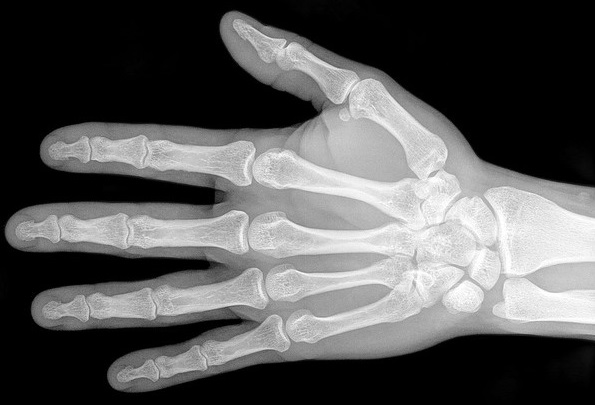
\includegraphics[width=\linewidth]{img/xrayhand.jpg}
  \caption{X-ray image of a human hand. In this negative image, bones are
  lighter because fewer X-rays managed to get through them.}
  \label{fig:xrayhand}
\end{center}
\end{figure}

\subsection{History}
Radiography builds on the work of Wilhelm Konrad R\"ontgen, a German physicist
who produced and detected X-rays for the first time on November 8, 1895.
These X-rays (X for unknown) had the remarkable property of being attenuated at
different rates when passing through various materials. For example, bone
strongly attenuates the X-rays while soft tissue does much less so. R\"ontgen
also discovered that the radiation can be captured on a photographic plate, just
like regular light. He presented his findings in his paper ``On a new kind or
rays'' \cite{rontgen}. This discovery earned him the Nobel Prize in Physics in
1901.

Only two weeks after his discovery he produced the first X-ray photo of his
wife's hand, after which she reportedly exclaimed: ``I have seen my death!''.
Just a couple of months later, X-rays were already being used in a clinical
setting on patients.

Note that during this time, not much was known about ionizing radiation or
radioactivity. Only a year after the discovery of X-rays did Henri Becquerel
discover radioactivity. Well known scientists such as Ernest Rutherford and
Pierre \& Marie Curie performed several more years worth of research before
realizing the true danger of prolonged exposure to this type of radiation.

\subsection{Technical background}
To better understand the internal workings of imaging devices, we present a
simplified mathematical and physical background based on the book of prof.
Suetens\cite{suetens}. X-rays are simply a form of electromagnetic waves
consisting of photons with a wavelength $\lambda$ on the order of Angstr\o ms
($10^{-10}$m). The corresponding frequency $f$ places these rays firmly in the
ionizing part of the spectrum - that is, they can cause cancer.
\autoref{fig:spectrum} shows a schematic overview of the whole spectrum. The
energy of such a wave can be calculated with the following formula, where $c$
is the speed of light and $h$ is Planck's constant.

\begin{figure}[ht]
\begin{center}
  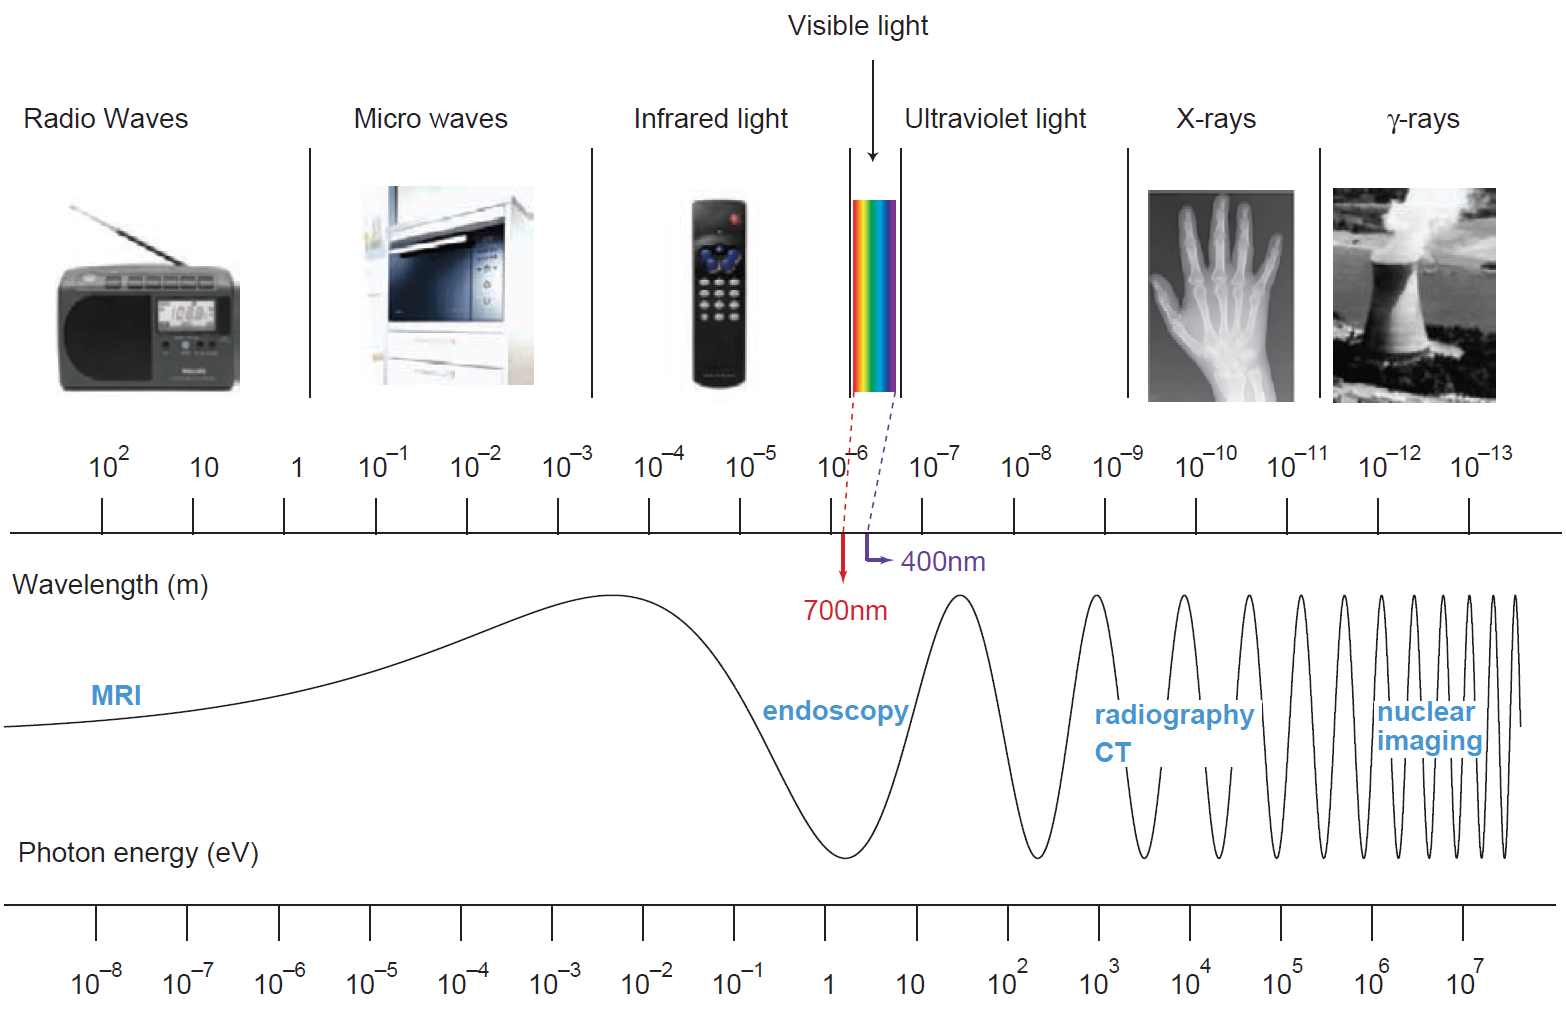
\includegraphics[width=\linewidth]{img/spectrum.png}
  \caption{The electromagnetic spectrum. \cite{suetens}}
  \label{fig:spectrum}
\end{center}
\end{figure}

\begin{equation}
	E = hf = \frac{hc}{\lambda}.
\end{equation}

X-rays are generated in an X-ray tube, a vacuum tube consisting of a cathode and
an anode. Current flowing through the cathode releases electrons,
which are accelerated toward the anode by an applied voltage. Once the electrons
hit the anode, they release part of their energy in the form of X-ray photons.
Thus, the two most important settings of an X-ray scan are the applied
current multiplied by the exposure time (mA $\cdot$ s) and the applied voltage
(keV).

The attenuation of X-rays through materials can easily be modeled using an
attenuation coefficient $\mu$. The beam intensity when passed through a
homogeneous material of depth $d$ is given by: 

\begin{equation}
	I_{out} = I_{in} \cdot \exp (-\mu d).
\end{equation}

This formula can of course easily be extended to include heterogeneous materials
and variable attenuation coefficients.

To capture X-rays, a detector is needed. Traditionally, a screen-film detector
was used. The familiar photographic film alone is very inefficient
at capturing X-rays: only about 2\% of all photons are absorbed. Because X-rays
are ionizing, the applied dose cannot simply be increased to improve the
image quality. Instead, an intensifier screen is used in front of the film. This
screen contains heavy chemical elements, whose electrons are excited by the
incoming photons. When returning to their original state, these electrons emit
visible light that can be captured more efficiently by the film, raising the
absorption rate to about 50\%.

Besides ordinary radiography, special classes such as fluoroscopy and
mammography exist. Fluoroscopy generates time-lapse recordings instead of still
images. With modern technology, tens of frames per second are achievable. Of
course, each frame must be shot at a very low exposure rate to minimize patient
risk. Mammography on the other hand produces images of the human breast. The
challenge here is to generate very high resolution images, so that small masses
can be seen.

\subsection{Recent advancements}\label{ssec:recentradio}
Relatively recently, X-ray systems have moved away from analogue detectors
towards digital ones. Much like digital photographs, digital X-ray scans are far
easier to store, copy, post-process and share. On top of that, they typically
have a much wider exposure range making them more tolerant to over- and
underexposure. These detector systems use storage phosphors to temporarily hold
the absorbed radiation instead of immediately releasing it in the form of
photons. This phenomenon is caused by electron traps in the doped material.
Later, this phosphor can be read out pixel-wise using an optical detector array
and a laser that gives the electrons enough energy to escape their trap. The
main obstacle for this paradigm shift was the large pixel size. Large pixels
translate to lower resolution, which is turn leads to a loss of diagnostic
value. Only by the time pixels could be as small as 0.1 mm did the medical world
embrace digital detectors \cite{review}.

Even newer devices use active matrix flat panel detectors. These detectors are
able to produce near real time images. In comparison, storage phosphors and
older technologies required minutes or more of processing time.

\subsubsection{A note on image quality}\label{sssec:imgquality}
The quality of an image can be expressed in three dimensions: resolution,
contrast and noise \cite{suetens}.

Resolution is sometimes simply stated as the pixel density (dots per inch).
However, this only provides an upper bound because in practise neighbouring
pixels are often correlated. For example, due to the imperfect nature of the
recording equipment, a single point can appear as blurred blob on the resulting
image. This blob is called the Point Spread Function (PSF), and is a better
measure for the actual image resolution. If the resolution is isotropic, the
Line Spread Function (LSF) - measured in distinguishable line pairs per
millimeter (lp/mm) - can also be used. Alternatively, the Optical Transfer
Function (OTF, sometimes also called MTF) representing amplitude and phase
shifts of a sinusoidal target can be used. In fact, this OTF is nothing more than the
Fourier transform of the PSF or LSF.

Second, contrast is the intensity difference between neighbouring regions of the
image. More formally, contrast at a given frequency is the amplitude component
of the image at that frequency in the frequency domain (calculated using the
Fourier transform). Contrast is dependent on the whole imaging process, but also
on the size and shape of the objects in the image. 

Third, noise is partly the result of interfering phenomena. Yet, it is also
inherent to the electromagnetic radiation itself because the waves themselves
are stochastic processes. An important measure is the Signal to Noise Ratio
(SNR) or, more appropriately, the Contrast to Noise Ratio (CNR). Noise can be
estimated by examining the result of an scan with no object present, a so-called
flat-field image. Another measure for the amount of noise is the Wiener
spectrum.

Another frequently used metric called the Detective Quantum Efficiency (DQE) can
compare various technologies without being dependent on the object being imaged.

\begin{equation}
DQE(f) = \frac{SNR(f)_{out}^2}{SNR(f)_{in}^2}
\end{equation}

In addition to these elements, sometimes artifacts appear on scans. The
causes of these artificial image features vary widely depending on the image
modality used and can also be caused by excessive post-processing.

\subsection{Future expectations}
Ever since CT scanners - and to a lesser extent MRI scanners - made their way
into hospitals, they have taken over many of the tasks traditionally reserved
for basic radiography. This declining trend is expected to continue in the
foreseeable future.

\section{X-ray computed tomography}
One step up from basic radiography is computed (axial) tomography (CT, formerly
CAT). The goal here is to create image slices of patients in the cross-sectional
plane rather than the frontal plane (tomography is Greek for ``slice writing'').
To accomplish this, the X-ray source-detector pair is rotated around the
patient. From this raw data, a so-called filtered back projection algorithm can
reconstruct the whole cross section image. A computer is needed to make sense of
the output, hence the \emph{computed} in the name. \autoref{fig:ctscan} shows an
example of a chest CT scan and \autoref{fig:ctscanner} shows an actual scanner.

\begin{figure}[ht]
\begin{center}
  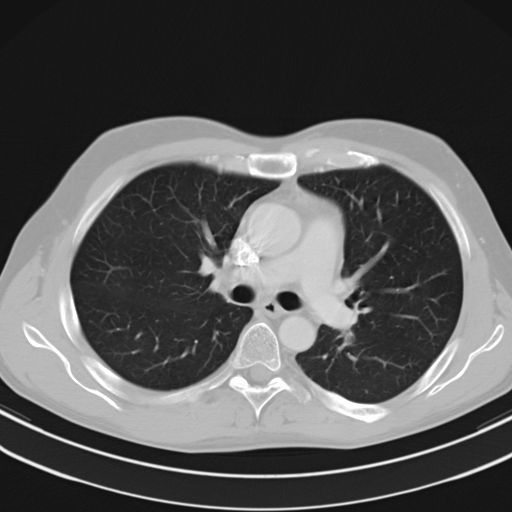
\includegraphics[width=0.4\linewidth]{img/ct-thorax.jpg}
  \caption{Example of a thoracic CT scan. The heart is clearly visible in the
  center. Bones (ribs, sternum, spine) are also easy to spot in the periphery.
  The large black area represents the lungs filled with air.}
  \label{fig:ctscan}
\end{center}
\end{figure}

\subsection{History}
Before computed tomography became possible, some simpler techniques were already
being used to obtain slices from inside the patient's body. These techniques
were called (non-computed) tomography. One example is linear tomography,
where source and detector move on parallel tracks, but in opposite directions,
during the scanning process. This way, one section of the patient is always
projected on the same spot of the detector, while the rest is averaged out.
Obviously, these techniques where nowhere near as accurate as the CT scanners we
know today.

In 1917, Johann Radon - an Austrian mathematician - presented the first
algorithm to reconstruct a function from its projections: the Radon transform
\cite{radon}.

After World War II, the development of computers gained momentum, but it would
still take a long while before the ``computed" in ``computed tomography" became
feasible. In the 1960's, the South African Allan McLeod Cormack continued
working on the mathematics invented by Radon \cite{ctreview}. A decade later, in
1972, the first operational brain CT scanner (the EMI scanner) was designed by
Godfrey Hounsfield, an Englishman. A scan took about 5 minutes, after which a
computer performed calculation for up to 150 minutes. The final output was a
80px $\times$ 80px image. Cormack and Hounsfield shared the 1979 Nobel Prize in
Physiology or Medicine for their work related to CT scans \cite{ctbook}.

\begin{figure}[ht]
\begin{center}
  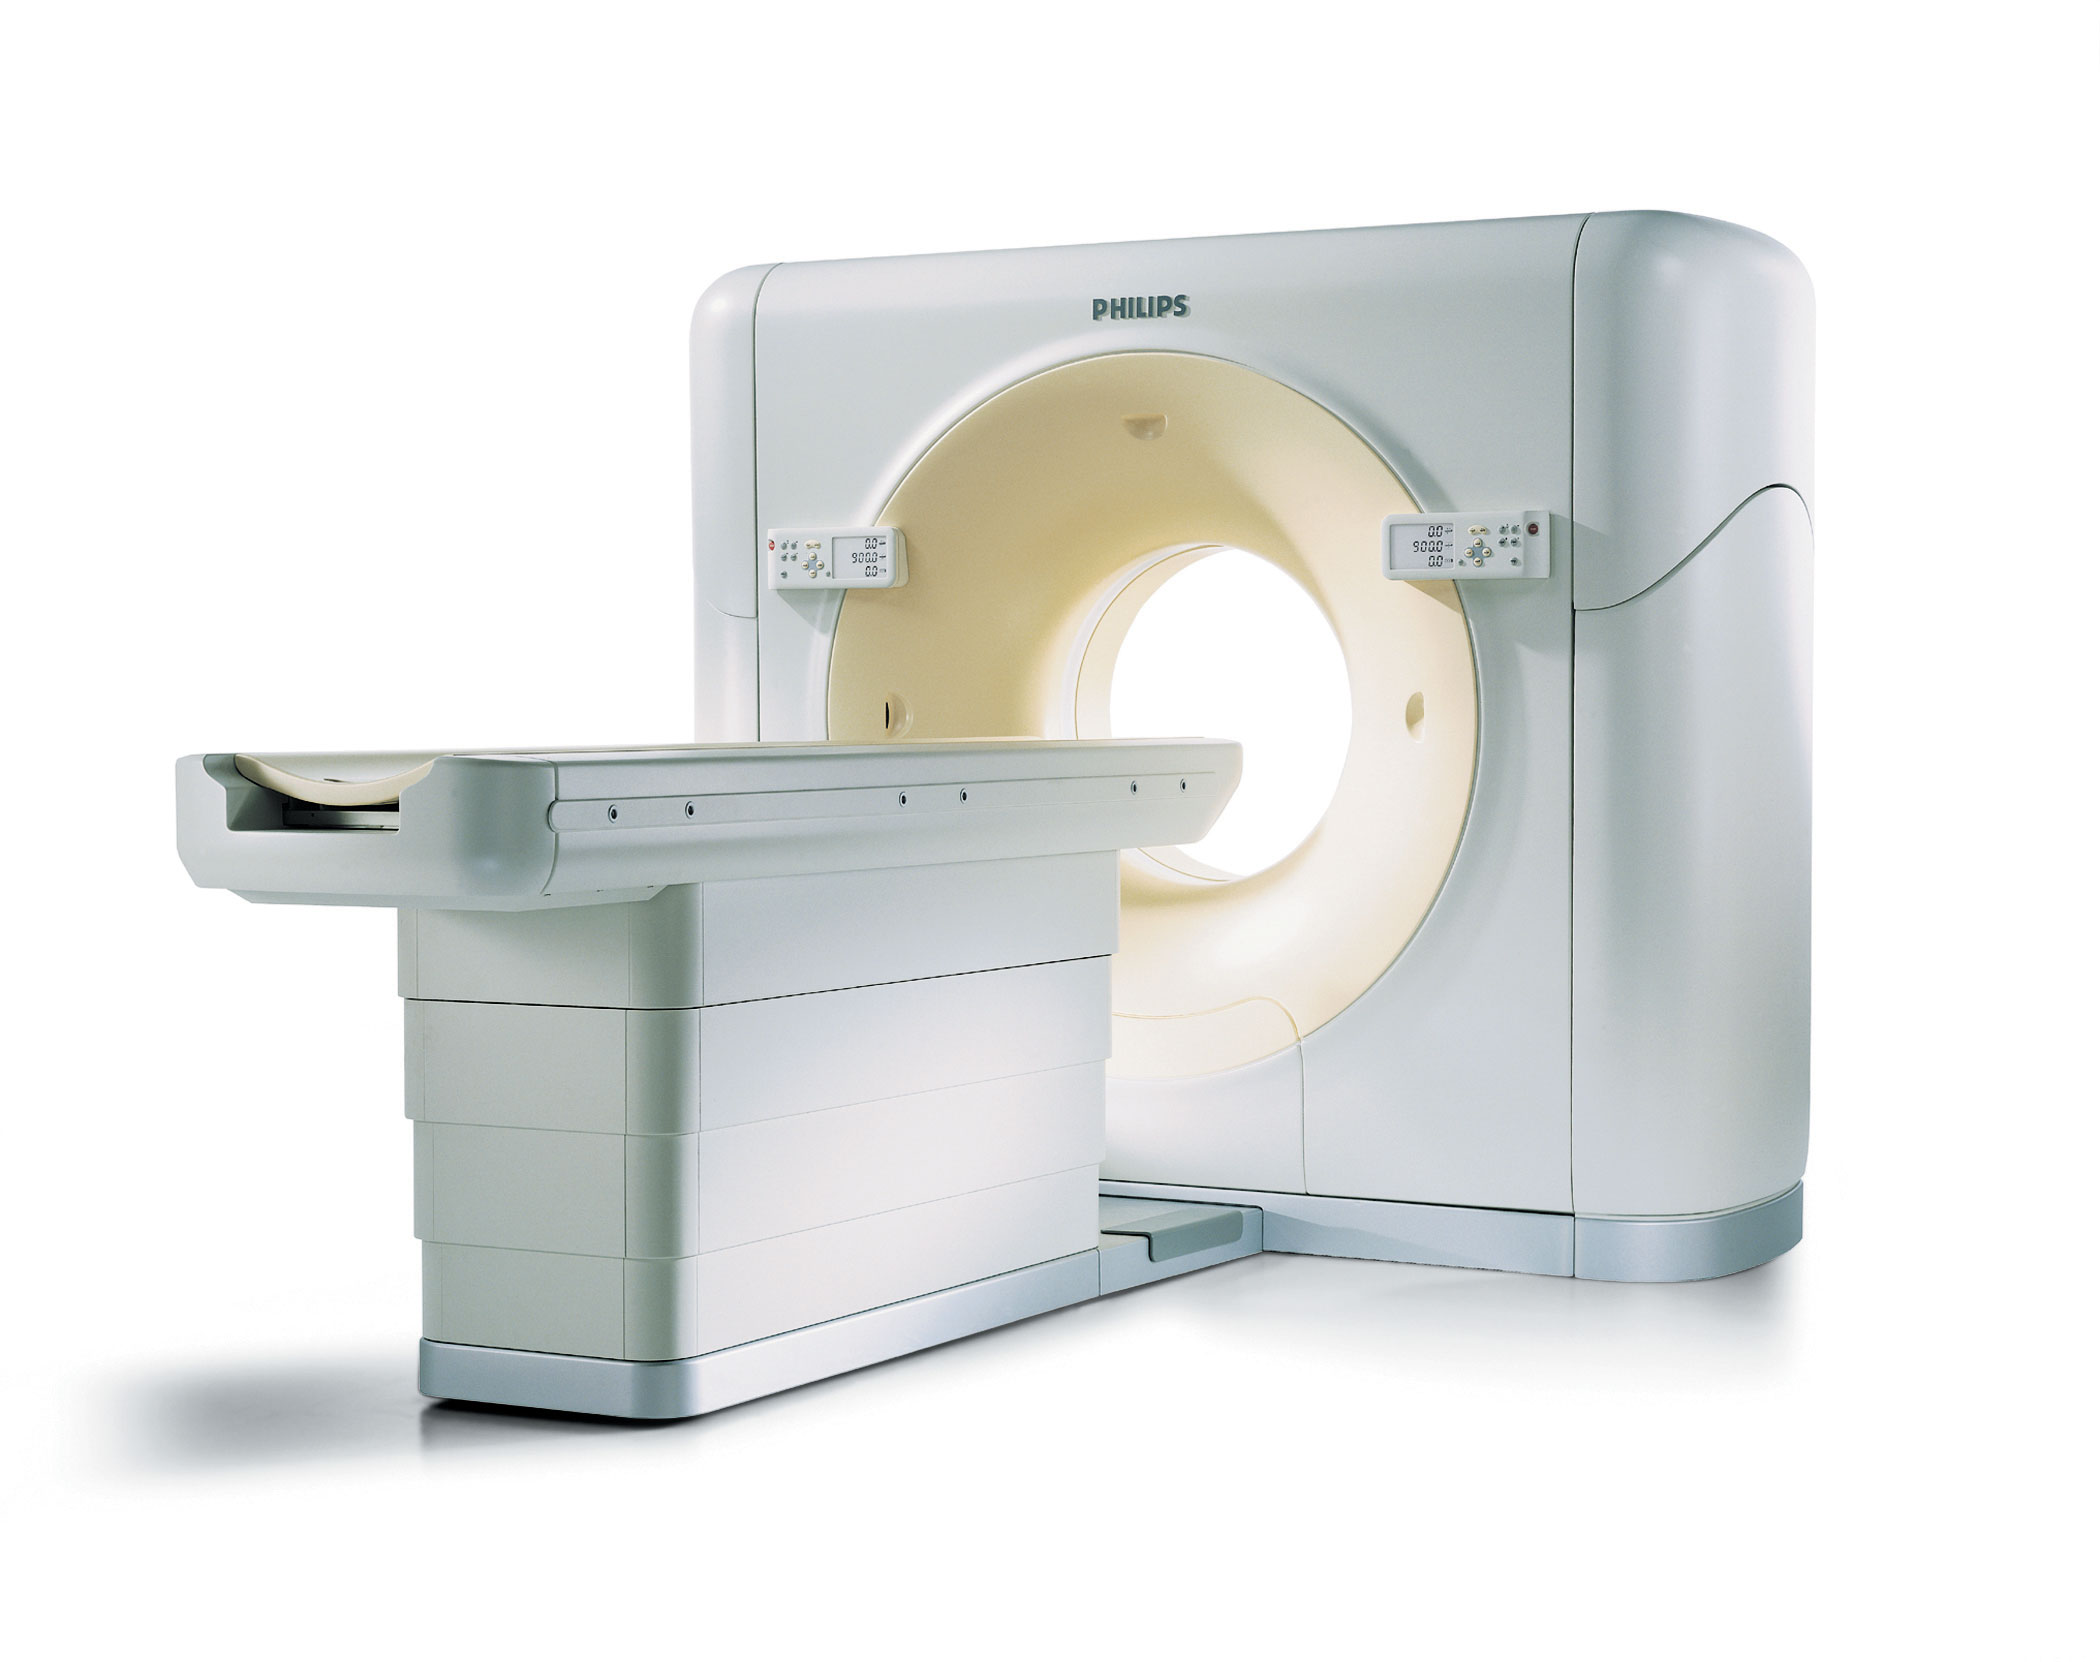
\includegraphics[width=\linewidth]{img/ctscanner.jpg}
  \caption{A CT scanner made by Philips. The patient takes place on the table
  and slowly slides through the toroid wherein the rotating X-ray
  source-detector pair is embedded.}
  \label{fig:ctscanner}
\end{center}
\end{figure}

\subsection{Technical background}
Just like radiographs, CT scanners are based on X-ray technology. They also
require a source and a detector, but this time they can rotate along the
patient. For every rotation angle $\theta$, we obtain an intensity profile
$I_\theta(r)$ along the axis $r$ perpendicular to the incoming X-rays (with
uniform incoming intensity $I_0$). The family of functions $I_\theta$ can be
transformed into an attenuation profile $p(r, \theta) = -\ln \tfrac{I_\theta(r)}{I_0}$
(often called a sinogram). This $p(r, \theta)$ is called the Radon transform of
the attenuation distribution $\mu(x,y)$ in the slice plane.
\begin{equation}
	p(r, \theta) = \mathscr{R}\{ \mu(x,y) \}
\end{equation}

In short, the projections $p$ is what we can measure (or at least sample at
fixed intervals) and the attenuation distribution $\mu$ is what we are
interested in. The mathematics required to go from the latter to the former are
pretty straightforward, but the reverse is more complicated. The inverse Radon
transform $\mu = \mathscr{R}^{-1}(p)$ is needed.

We will not go into details, but the solution lies in the projection theorem.
This theorem states that the 2D Fourier transform $M(k_x, k_y)$ of $\mu(x,y)$
is equal to the 1D Fourier transform $P(k, \theta)$ of $p(r, \theta)$ (save for
a simple polar coordinate transformation).

\begin{equation}
\mathscr{F}_{1D}\{ p(r, \theta) \} = P(k, \theta) = M(k \cos \theta, k \sin
\theta) = \mathscr{F}_{2D}\{ \mu(x, u) \}
\end{equation}

Because the inverse Fourier transform is well understood, we have a solution to
our problem. Simply calculate $P$ from $p$ as explained above, and then apply
the inverse 2D Fourier transform to obtain $\mu$. By using the polar version of
the Fourier transform, we can reduce artifacts. This approach is called filtered
back projection \cite{suetens}.

After all the calculations are performed, we typically acquire a 512px $\times$
512px scan. The values of the pixels in a CT scan are referred to as the CT
numbers and are expressed in Hounsfield Units (HU). They are calculated using
the fomula below, where $\mu$ is again the attenuation coefficient.
\begin{equation}
	\text{CT number} = \frac{\mu -
	\mu_{\text{H}_2\text{O}}}{\mu_{\text{H}_2\text{O}}} \cdot 1000
\end{equation}

From this, it becomes obvious that the CT number of air (with $\mu = 0$) is
-1000 HU and that the CT number of water is 0 HU. Bones on the other hand have a
very high attenuation coefficient and thus have a CT number in the thousands.
Soft tissue lies somewhere in between.

\subsection{Recent advancements}
The previous section assumed parallel X-ray beams. However, newer generation
scanners often employ cone-shaped beams. The procedure outlined above can
reconstruct a single slice by rotating around the subject by 180 degrees at a
time (a circular CT). On the other hand, modern CT scanners often spiral around
the patient while he moves through the toroid (a helical CT) to speed up the
process and thus decrease the exposure. Another useful trick is to capture
multiple slices at once by using multiple detector arrays. Until recently,
manufacturers were in a so-called \emph{slice wars} to offer the most detector
arrays. Needless to say, all this substantially complicates the mathematics
required to perform a back projection, but it is feasible and daily used in
hospitals around the world.

Another point of interest today is the combination of successive CT slices to
generate a 3D model of the patient. Because of advancements in computer
technology and algorithms, we can now post-process this 3D model to
automatically segment the organs and other structures. This can for example help
physicians plan their actions before and during complex surgery.

\subsection{Future expectations}
Because CT scanners still require relatively high doses of radiation, this is
not an ideal solution. MRI scanners offer a safer alternative, but the large
magnetic fields produced make them impossible to use on patients with ferromagnetic
implants. Another advantage over MRI is the superior sub-millimeter resolution
that only CT scanners can offer. These are only some of the reasons why they
will not be replaced anytime soon. Future research will attempt to make CT
scanners even faster and allow them to produce clearer (i.e., higher contrast)
images with lower doses.

\section{Magnetic resonance imaging}\label{sec:mri}
While the previous imaging modalities were based on X-rays, Magnetic Resonance
Imaging (MRI) is based on magnetic fields. It is sometimes also referred to as
Nuclear Magnetic Resonance (NMR) in professional circles. However, the general
public has a certain aversion to the world ``nuclear'', so MRI is more common.
Instead of measuring the electromagnetic attenuation properties of various
tissue types as in CT scanners, we measure certain magnetic properties of the
tissue. These magnetic properties mainly depend on the molecular composition of
the material, for example on the amount of H$^+$ ions present (the proton
density). These electromagnetic waves are non-ionizing, meaning they cannot
cause cancer due to prolonged exposure. The goal is the same: imaging slices of
a patient's body. While technically an MRI scanner can generate slices in any
orientation without even moving the patient, CT-like cross sectional slices
are still used predominantly. Figure \ref{fig:mriscanner} shows a picture of an MRI
scanner.

\begin{figure}[ht]
\begin{center}
  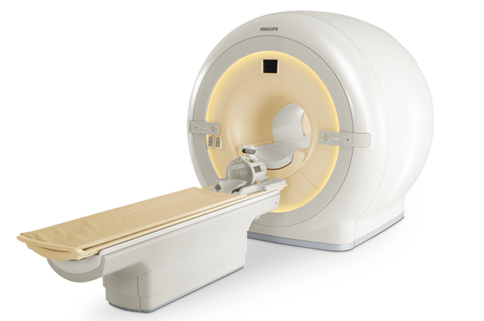
\includegraphics[width=\linewidth]{img/mriscanner.jpg}
  \caption{A Phlips MRI scanner. The patient takes place on the bed and is
  moved inside the toroid, but is not moved again during the procedure.}
  \label{fig:mriscanner}
\end{center}
\end{figure}

\subsection{History}\label{ssec:mrihist}
During the late 1960's, researcher in Aberdeen worked on the predecessor of the
modern MRI scanner \cite{mrihistory}. Their goal was to distinguish between
malignant tumors and normal tissue without using ionizing radiation. Instead of
measuring the magnetic properties of the nuclei, they initially focused on
electrons. This proved to be a dead end, and by early 1970 the group moved on to
NMR as we know it today. They realized that tumors have a longer $T_1$ time
(see below), and concentrated on that instead.

Meanwhile in the USA, chemist Paul Lauterbur proposed a way to create images
from NMR studies by using multiple field gradients to encode the position of
each measurement \cite{lauterbur1973}. Another important contribution came from
Peter Mansfield (now Sir), an English physicist. In 1974, he showed how to
select spins from a specific slice and patented a method to selectively excite
and define a slice across a sample. Lauterbur and Mansfield shared the 2003
Nobel Prize in Physiology or Medicine for their work on NMR.

From 1978 on, multiple research groups started presenting images generated by
prototype MRI scanners. However, only in the early 1980's was the technology 
ready for clinical and diagnostic use. By 1983, major multinational corporations
started producing commercial MRI machines.

\subsection{Technical background}
Unfortunately, the fundamental concepts that make MRI scanners work go beyond
classical physics, and instead requires special relativity, quantum mechanics
and quantum electrodynamics. Clearly, this is way beyond the scope of this text. We
will present a simplified version of the core principles based on
\cite{suetens} instead.

MRI scanners influence and measure the magnetic properties of atom nuclei in the
patient's tissue. During typical studies H$^+$ ions (i.e., protons) are used
because of their abundance in the human body, although alternatives exist
(e.g., ${}^{13}_6$C or ${}^{17}_8$O).

When the scanner is operational, a large magnetic field $\vec{B_0} = (0,0,B_0)$
(in the order of a couple Telsa) is induced along the patient's length using a
big electromagnetic coil. By supercooling the coil, the resistance drops and
power consumption can be reduced significantly.

The magnetic field $\vec{B_0}$ influences the magnetic moments $\vec{\mu_i}$ of
the nuclei, causing them to precess around the z-axis with precession frequency
$\omega_0 = f(B_0)$. Associated with the external magnetic field and the
individuel magnetic moments is the potential energy $E$. Quantum mechanics
states that for protons, this energy can only have two values, the so-called
spin up ($E_\uparrow$, lowest) and spin down ($E_\downarrow$, highest) state. In
these states, the $\vec{\mu_i}$ point respectively upwards ($\mu_{iz} > 0$) and
downwards ($\mu_{iz} < 0$), although transverse components are still present.
Most protons will be in the lowest energy state, but they can be flipped by absorbing
a photon with the appropriate amount of energy $\Delta E = E_\downarrow -
E_\uparrow$. This holds when the photon has a specific Larmor frequency
$\omega_{RF}$, which happens to be equal to $\omega_0$. In a 1.0T magnetic
field, the Larmor frequency for hydrogen is 42.6 MHz, a radio-frequency (RF) wave.

Of course, we are more interested in macroscopic voxels (3D pixels) than in the
individual nuclei. Fortunately, the net magnetization vector of each voxel is
simply the sum of all individual magnetic moments: $\vec{M_0} = \sum_i
\vec{\mu_i}$. The magnitude of this vector roughly represents the proton density
in the voxel. In dynamic equilibrium, $\vec{M_0}$ points in the same direction
as $\vec{B_0}$ because there are more nuclei in the spin up state and the
individual transverse components cancel each other out. To summarize: the large
magnetic field make sure the net magnetization vectors of all voxels are
aligned.

Unfortunately, due to technical reasons we can only measure the transverse
component of $\vec{M}$. As a solution, we will disturb the dynamic equilibrium
with a resonating RF pulse, causing more protons to flip to the spin down state.
This RF wave has a magnetic component $\vec{B_1} = (B_1, 0, 0)$. Following the
same logic as above, $\vec{B_1}$ causes $\vec{M}$ to precess around it. With the
appropriate timing, $\vec{M}$ can be flipped over an angle $\alpha$ of either 90
or 180 degrees.

After the pulse, the system returns to dynamic equilibrium during a process
called relaxation. We can distinguish between two effects. First, spin-spin
relaxation is responsible for the disappearance of the transverse component of
the net magnetization vector due to loss of phase coherence (increase in
entropy while energy stays constant). This process can easily be approximated
by a first order model with a time constant $T_2$, called the spin-spin
relaxation time.

\begin{equation}
M_{tr}(t) = M_0 \sin(\alpha) \exp\left(\frac{-t}{T_2}\right)
\end{equation}

Different tissue types have different inherent $T_2$ times, which we will
exploit later.

\begin{figure}[ht]
\begin{center}
  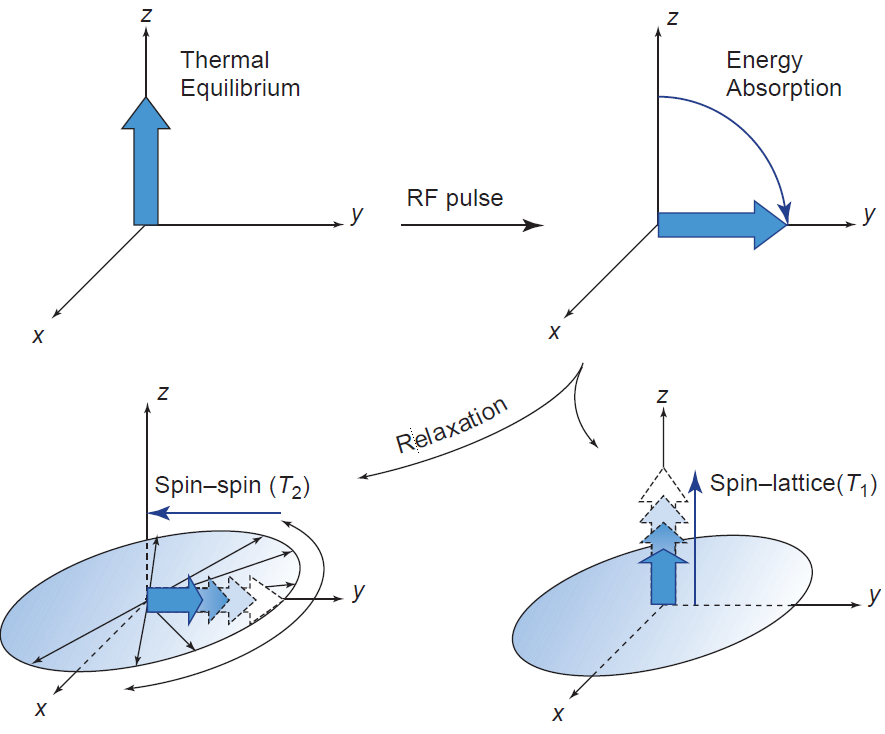
\includegraphics[width=\linewidth]{img/relaxation.png}
  \caption{Schematic overview of relaxation after a 90 degree pulse. \cite{suetens}}
  \label{fig:relaxation}
\end{center}
\end{figure}

Second, spin-lattice relaxation is responsible for regenerating the
longitudinal component of $\vec{M}$. Similarly, this process can be linked to a
$T_1$ relaxation time. $T_1$ is also a tissue property, and is always larger
than $T_2$.

\begin{equation}
M_l(t) = M_0 \cos(\alpha) \exp\left(\frac{-t}{T_1}\right) + M_0 \left(1 -
\exp\left(\frac{-t}{T_1}\right)\right)
\end{equation}

Using a quadrature detector in the xy-plane, we get the following reading
after one 90 degree pulse:
\begin{equation}
s(t) = M_{tr}(t) = M_0 \exp\left(\frac{-t}{T_2}\right)
\end{equation}

To also measure $T_1$, we have to repeat the 90 degree pulse after repetition
time TR:
\begin{equation}
s(t) = M_0 \left(1 - \exp\left(\frac{-TR}{T_1}\right)\right)
\exp\left(\frac{-t}{T_2}\right)
\end{equation}

Notice how the 90 degree pulse conveniently eliminates the sine and cosine
factors.

Clearly the result is not just the proton density $M_0$, but involves other
factors as well. This is not necessarily a problem as the $T_1$ and $T_2$
factors can increase the discriminative power of the scanner. If a short $TR$ is
chosen, the image is said to be $T_1$ weighted because long $TR$ times cause the
$T_1$ factor to diminish. If on the other hand a long $TE$ (echo time = moment
of measurement) is chosen, the image is said to be $T_2$ weighted. Indeed, a
short $TE$ time decreases the $T_2$ factor. By combining a long $TR$ with a
short $TE$, we have a relatively pure proton density image. Remember that $TR$
and $TE$ can be chosen by the operator, while $T_1$ and $T_2$ are tissue
dependent.

The attentive reader will have noticed that there is no spatial information
encoded in this signal yet. Using this approach we could only measure the
combined effects of all relaxations, which is useless. To solve this, we
superimpose additional gradients $\vec{G}_{x/y/z}$ (in the order of
milliTesla/meter) onto $\vec{B_0}$. This in turn affects the Larmor frequency.
The exact details are far from trivial and will be omitted, but involve the
3D k-space. After the signal has been sampled everywhere in the region of
interest in the k-space, a simple inverse Fourier transformation yields the
image we are looking for.

Using two 90 degree pulses is just one of the many possible pulse sequences used
in modern MRI scanners. Other examples include the spin-echo (SE) sequence and
the gradient echo (GE) sequence. Each sequence has advantages and disadvantages
with respect to discrimination of certain tissue types. The radiologist is
responsible for making the proper choice.

%fMRI (oxygen T2)
%flexible

\subsection{Recent advancements}
A lot of spin-off technologies based on MRI are in use. For example, Magnetic
Resonance Angiography (MRA) generates images of arteries to detect pathologies
such as stenosis (narrowing) or aneurysms (dilations). To make this work the
patient can be injected with a paramagnetic contrast material. Alternatively,
the scanner can detect anomalies in the measurements due to movement of the blood, and
amplify those.

\hyphenation{me-ta-bo-lites}

Similarly, Magnetic Resonance Spectroscopy (MRS) measures the levels of various
metabolites in human tissue, while functional MRI (fMRI) visualizes brain
activity based on local oxygen levels. The underlying principle is that
oxygen-rich blood contains oxyhemoglobin, which is diamagnetic, while
oxygen-poor blood containing deoxyhemoglobin is paramagnetic. Likewise,
diffusion and perfusion can be measured.

\subsection{Future expectations}\label{ssec:mrifuture}
MRI scanners today are still far less ubiquitous than CT scanners, and only make
up a few percent of the worldwide radiographic examinations \cite{oecdhealth}.
However, because of the various advantages over other modalities - mostly the
fact that it is not dependent on ionizing radiation - usage is expected to
rise steadily in the future. MRI will never completely replace CT because it cannot properly
image hydrogen-poor structures such as bone and air.

On top of that, future research will most likely improve the functional aspect
(e.g. measuring blood flow) of MRI. This can be done by experimenting with
nuclei other than hydrogen, by using new contrast agents and using novel pulse
sequences. In addition - similar to CT scanners - research will try to increase
the contrast and lower the acquisition times even further.

\section{Nuclear medicine imaging}\label{chap:nuclearimg}
While the previous imaging modalities mostly focused on obtaining static images
of the patient, nuclear medicine imaging concentrates on so-called functional
imaging: visualizing some kind of dynamic process (e.g. drug metabolism) in the
human body. CT or MRI scanners also have this capability by exploiting certain
side effects of their underlying phenomena, but the Signal to Noise Ratio (SNR)
is always significantly lower.

Diagnostic nuclear medicine imaging works by tracking radioactive isotopes
(tracers) as they move through the body. A distinction can be made between two
kinds of radiopharmaceuticals. One type is simply meant to spread through the
body, and is expected to have some default, static distribution after a
sufficient amount of time has passed. Contrast agents used in CT and MRI scans
fit this description rather well. Physicians can compare the actual
distribution with the expected distribution, and take the differences into
account when coming up with a diagnosis. The other type of radiopharmaceuticals is used
in nuclear medicine, and is more dynamic. Here, we are not interested in some
static distribution, but in specific movements of the tracer over time. These
movements are intended to be correlated with some kind of biochemical or
physiological process in the human body. Unlike with the former type, the latter
type does not require high quality images to be effective. Rather, the fidelity
of the tracer used is paramount \cite{radiopharma}.

In the early days hospitals needed their own cyclotron to produce these tracers,
which significantly slowed adoption. Nowadays various companies deliver the
needed tracers daily to hospitals around the world \cite{petreview}. Other
variants of nuclear medicine are used in the oncology departments to fight
cancer, but we will not go deeper into that.

Two main scanner types fall under nuclear medicine imaging: Positron Emission
Tomography (PET) and Single Photon Emission Computer Tomography (SPECT). The
exact difference will be explained later on in the technical background section.
\autoref{fig:petscanner} shows an example of a PET scanner.

\begin{figure}[ht]
\begin{center}
  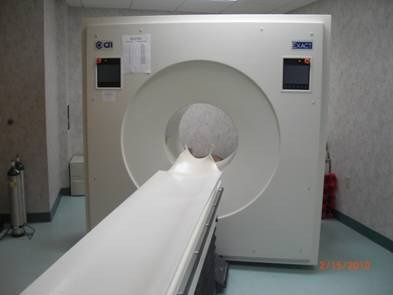
\includegraphics[width=\linewidth]{img/petscanner.jpg}
  \caption{A PET scanner made by Siemens. The opening is completely surrounded
  by detectors, so there are no moving parts inside.}
  \label{fig:petscanner}
\end{center}
\end{figure}

\subsection{History}
The history of nuclear medicine begins with the work of German physicist Hans
Geiger, a student of Ernest Rutherford, and his 1908 invention: the Geiger
counter. This device can detect ionizing radiation by exploiting the fact that
these rays can make an inert gas (e.g. Argon) conduct electricity. Using
this rudimentary device, researchers could form a rough picture of the radioactive
activity in a patient's body \cite{specthistory, geigercountertube}.

Meanwhile, Paul Direc, an English theoretical physicist, laid the theoretical
foundation for what would later be known as a positron.\cite{positrontheory}.
Around the same time, Fr\'ed\'eric Joliot and Ir\`ene Curie (daughter of Pierre
and Marie Curie) dicovered artificial radioactivity \cite{artificialradio}.

A significant breakthrough came with the invention of the Anger camera (or
gamma camera) in 1957 by Hal Anger, an American engineer and physicist. This
camera was able to detect incoming radiation from a whole organ at once,
improving the spatial resolution dramatically. The technique he used was based
on scintillator crystals \cite{anger}.

From there, several researchers such as Crandall, Cassen, Kuhl and Edwards built
upon the work to create true scanner systems throughout the late 1960's and
early 1970's. The first systems were SPECT scanners to make images in just one
plane, and later on CT-like scanners that could calculate cross sections were
invented.

Research concerning PET scanners was performed at about the same time
as SPECT scanners. Scientists soon realised their advantage, but adoption took
much longer in comparison \cite{petreview}. G. Brownell and his group were the
first to build a working dual planar PET scanner \cite{brownell}. Only since
1990 have PET scanners seen significant clinical usage \cite{pethistory}.

\subsection{Technical background}
Before we explain how PET and SPECT scanners work, we will quickly refresh some
important radioactive decay modes.

The first is positron emission, also called $\beta^+$ decay. Positrons (e$^+$)
are the anti-particles of electrons (e$^-$). During this decay, a proton (p$^+$)
inside an atom is essentially transformed into a neutron (n) and a positron.

\begin{equation}
	p^+ \rightarrow n + e^+
\end{equation}

\begin{equation}
	{}_Z^AX \rightarrow {}_{Z-1}^AY + e^+
\end{equation}

In the next couple of picoseconds, the positron will fly into a electron and
annihilate. The mass of the two particles is is converted into pure energy in
the form of two photons ($\gamma$). Using Einstein's famous equation $E = mc^2$,
we can calculate that each photon carries 511 keV of energy. They fly away in
opposite directions.

This physical phenomenon forms the basis of Positron Emission Tomography (PET).
A typical element used during such studies is $^{18}$F, which has a half-life of
about 110 minutes. It almost exclusively decays by positron emission and yields
stable $^{18}$O \cite{suetens}. The radioactive element is typically coupled to
another molecule to facilitate uptake and transport in the body. One commonly
used molecule is Fluorodeoxyglucose (FDG), which binds to fluorine-18 and is
used to visualize glucose metabolism.

The fact that two photons are emitted in opposite directions is very convenient.
If both happen to be detected, we immediately know their projection line.
(Remember that in CT scanners the projection line is known a priori and is fixed
between source and detector.)

The opposite operation is also possible: $\beta^-$ decay by electron emission.
Here, a neutron is converted into a proton and an electron.

\begin{equation}
	n \rightarrow p^+ + e^-
\end{equation}

\begin{equation}
	{}_Z^AX \rightarrow {}_{Z+1}^AY + e^-
\end{equation}

In certain cases, the resulting Y atom is in a metastable state ($^{Am}$Y).
This means the atom will later decay further into a more stable nuclear
configuration, releasing one or more photons in the process. This is much more
interesting diagnostic-wise, because unlike electrons, photons don't damage the
tissue they pass through during emission. A common metastable element
used is $^{99m}$Tc, generated after decay of $^{99}$Mo and further decaying
into $^{99}$Tc (half-life of six hours) by emitting a single photon of 140 keV.

$\beta^-$ decay is mainly used in SPECT scanners. Because only one photon is
emitted, we cannot immediately tell where it came from when it is detected. To
solve this, a mechanical collimator - a thick lead plate with holes in it - is
used to absorb all photons that do not approximately fly perpendicular to it.
Knowing this, we can estimate the projection line of the photons we managed to
detect after they passed through the plate. Sadly, this technique forces us to
make a trade-off between spatial resolution (using smaller holes) and
sensitivity (letting more photons through using bigger holes). This is a serious
disadvantage compared to PET, in turn making SPECT less future-proof.

Note that these photons form electromagnetic waves, and their frequencies are
equal to or higher than those of the X-rays in earlier sections. This means that
they obey the same physical laws, and thus they also attenuate when passing
through tissue. However, in this context we refer to the radiation as
$\gamma$-rays instead.

When the photons are detected and the projection lines are calculated, we have
two options. Either we are satisfied with planar imaging to get a result similar
to basic radiography. In this case all depth information is lost, and the pixels
simply give information about the photon emission activity on their entire
projection line, combined with the attenuation properties of tissue on that
line. Sometimes a SPECT scanner is simply called a gamma camera in this
configuration, although the distinction is mostly theoretical. The other option
is to use a slightly adapted filtered back projection algorithm to compute
CT-like slices. Obviously this requires the detectors to rotate about the
patient just like in a CT scanner.

The detectors used here differ significantly from those used with X-rays. Not
only are there far fewer photons to be detected in the first place, but the
acquisition time is also much longer. Photomultiplier Tubes (PMT) combined with
NaI(Tl) scintillator crystals and, more recently, photo diodes are popular
detectors for use in SPECT scanners today. PET scanners on the other hand use
materials such as Bismuth Germanate (BGO) and Lutetium Oxyorthosilicate (LSO) in
their detector scintillators.

\subsection{Recent advancements}
Due to the strong attenuation of the photons, filtered back projection produces
significant artifacts in the final image. The images are still diagnostically
relevant, but better methods are available. Iterative reconstruction based on
Bayesian statistics or maximum likelihood calculations are becoming more
popular \cite{suetens}.

Another advancement, the Time-of-Flight (TOF) PET scanner, estimates the
source location of the photon along the projection line by measuring the
difference in arrival time between the two photons. This only works reliably if
the difference is smaller than 1ns, which in turn requires very advanced measuring
equipment.

While most researchers focus on nuclear medicine alone, others seek their
fortune in hybrid scanners. For example, combining CT or MRI with PET or SPECT
scanners significantly improves the specificity compared to their stand-alone
versions. Especially the PET/CT combination is popular in clinical environments.
In this case, the CT scanner can provide the attenuation correction needed for
the PET scanner. One problem that has to be overcome is the long acquisition
time needed for PET, and the mismatch it causes with CT scans due to patient
movement. Image registration techniques can be helpful here, but are not
straightforward.
\ldots

\subsection{Future expectations}
As with all types of scanners, we expect steady technological advancements in
the years and decades to come. However, in the case of nuclear medicine, experts
expect most progress to be made on the tracer front. This will enable researcher
to not only visualize biological processes on a macro level, but move to the
molecular level. This way, advanced studies on gene regulation, radio
immunotherapy etc. will become possible.

\section{Computer-aided Detection and Diagnosis}
This section on Computer-aided Detection and Diagnosis (CAD, not to be
confused with Computer-aided Design) deals not with the image creation process,
but with the subsequent processing. In this sense it is the odd one out.

CAD is one of the major research areas in diagnostic medical imaging
\cite{cadhistory, suetens}. CAD technologies help radiologists with the actual
detection and diagnosis of pathologies in the image. Sometimes a further
distinction is made between detection (CADe) and diagnosis (CADx). Either way,
CAD does not attempt to replace physicians. You can think of it more as a second
opinion. This is in contrast with Automated Computer Diagnosis (ACD) where the
computer (supposedly) does all the work and no physician is needed anymore.

The rise of CAD is tied to the increased workload of radiologists. Decades ago,
each radiological examination contained just a few images. Today, with
multi-slice CT scans and full body MRI scans, a single examination can contain
thousands of 2D images. Clearly, some form of automation would be more than
welcome to reduce the radiologists' workload.

A (non-exhaustive) list of possible application of CAD include detection of
vertebral fractures on radiographs, detection of microcalcifications on
mammograms, detection of cranial aneurysms in MRA images and detection of lung
nodules in CT scans \cite{cadhistory}.

Note: in the following sections related to CAD, we assume that the reader is
familiar with the basics of statistical binary classification theory. The most
important concepts are True Positives (TP), False Positives (FP), True Negatives
(TN), False Negatives (FN), accuracy, sensitivity and specificity.

%, and Receiver Operating Characteristic (ROC) curves.

%US4907156 \cite{chan1990method}

\subsection{History}
Early in the 1980's, when large scale research on CAD began, the most common
techniques fell under basic image processing. This is a branch of signal
processing, applied to 2D signals (i.e., images). In the following years, a new
field called Computer Vision formed around the subject. 

To get a feel for such image processing techniques, consider a special filter
to accentuate lung nodules, and another one to suppress them. Next, apply these
two filters to the same image, and subtract the suppressed from the accentuated
version. The result should then be a completely black image, save for the
nodule-like structures in the image. 

Early on, most research focused on ACD. It was not a success at first,
because computers were not yet powerful enough, and advanced image processing
algorithms were not yet available. The researchers had high hopes for the
future, but unfortunately ACD never caught on. The algorithms' sensitivity and
specificity simply did not match up to that of real physicians. That is why most
researchers soon made the switch to CAD. To measure the performance of CAD
systems, we do not only look at the outcome of the algorithm, but how this outcome
combined with the physician's expertise can create synergy. Even if the
sensitivity and specificity of the CAD algorithm are lower than that of the
average physician, as long as the synergy is big enough, their combined use can
trump that of the physician alone. This was proven for the first time in
\cite{cadsynergy}.

At the time, the most popular topics were related to cardiovascular diseases,
lung cancer and breast cancer because of their high impact. This trend has
largely continued, and even in recent year researchers still focus mostly on the
latter two topics. \cite{cadhistory}

The first scanner with built-in CAD detection was approved by the U.S. Food and
Drug Administration (FDA) in 1998.

\subsection{Technical background}\label{ssec:cadtech}
Contrary to the discussion of the previous imaging modalities, we will not go
into the technical details of these techniques. There reason is simple: there
are too many of them, and they all work in a very different way. The interested
reader is invited to read a book on the subject such as \cite{imgprocbook}.

Fortunately, most CAD systems follow a generic scheme, independent of the
underlying technology \cite{lungcadreview}. First of all, the organ of interest
(e.g., the lungs) is segmented (I), and the rest of the image is discarded.
Next, the object to be detected is somehow enhanced (II). The subtraction
technique outlined above could work here. Then, these candidate objects have to
be detected and segmented (III). After that, some kind of feature analysis is
performed and the candidates are properly classified (IV). Most techniques will
still have plenty of false positives at this point, so FP reduction is required
(V). If simple detection was the goal, the remaining candidates are the end
result of this scheme. Else, an extra diagnosis (characterization) step is
required (VI).

\subsection{Recent advancements}\label{ssec:cadadv}
In the last two decades, more and more interest has been generated about the
implementation of artificial intelligence (AI) and machine learning techniques
in CAD. Examples of such techniques include Discriminant Analysis (DA),
Artificial Neural Networks (ANN), Support Vector Machines (SVM) and decision
tree models such as Random Forests (RF) \cite{lungcadreview, ginneken}. The
exact details of each method are out of scope for this text, but fortunately
most can be treated as black boxes with highly similar in- and outputs. 

Machine learning always works in two phases. The learning phase and the
prediction phase. During the learning phase, a large number of class-annotated
sample images are provided from which the algorithm can infer the differences
between various classes. Examples of simple binary classes are tumors vs.
non-tumors or malignant tumors vs. benign tumors. Once training has completed,
an unannotated picture can be provided in the prediction phase. The algorithm
will then predict - based on its internal model - to which class it belongs.

Of course it is possible to use a complete image, pixel by pixel, as input.
However, this is computationally very expensive. Instead, features are typically
calculated to describe a certain region of interest in an image. Simple
features are the minimum, average and maximum intensity, but they can become
arbitrarily complex.

\subsection{Future expectations}
\cite{cadhistory} sees future potential of CAD in combination with Picture
Archiving and Communication Systems (PACS). Since the digital revolution,
hospitals had to come up with a new way of storing and managing all this imaging
data. PACS was the solution, and today every modern hospital has a PACS in one
form or another. This means every hospital sits on piles of old and unused
medical images. By combining CAD, AI techniques such as data mining and PACS,
research could gain a serious momentum boost and unforeseen applications could
pop up. Furthermore, integrating CAD as a PACS module would make it more
accessible and promote adoption.

Aside from that, researchers will keep working on the underlying algorithms.
This will hopefully bring steady improvements in performance.


\chapter{Overview of radical inventions}\label{chap:inventions}

\section{Introduction}
In this chapter, we perform the assessment of five inventions based on the
framework described in \autoref{chap:intro}. Chapter \ref{chap:imaging}
already described various breakthroughs in diagnostic medical imaging, but most of them
predate 1980. Fortunately researchers in the field have come up with plenty of
other innovations in the last thirty years, some of which will be detailed
below. We included one invention per imaging modality described, plus one more
related to computer aided detection and diagnosis (CAD).

For each innovation, a technological definition is provided wherein the purpose
or goal is outlined, and the components plus their interactions are explained
based on a thorough literature review. Next, the innovation is scored based on
the assessment sheet in \autoref{app:score}.

\section{Radiography invention: digital radiography}
A quick Google search on ``radiography breakthrough" suffices to show that
digital radiography is the most significant invention for basic radiography in
recent decades. As mentioned earlier in \autoref{ssec:recentradio}, digital
radiographs are much easier to store, copy, post-process and share compared to
their analogue siblings. Additionally, unlike radiographic film there is no potential
for over- or underexposure. Instead, the output can be rescaled as needed during
post-processing. Some techniques also allow for a reduced exposure of the
patient, minimizing the risk. The ubiquity of digital scanners these days prove
that the advantages outclass the disadvantages. However, these disadvantages do
exist. Analogue images have a very high inherent resolution, and by examining
them on a lightbox the contrast is unmatched by any kind of computer screen. In
addition, because analogue systems do not use digital electronics, there is no
electronic noise. Digital radiographs do not have necessarily to outclass their
analogue counterparts on these fronts, but they have to achieve a minimum level
to make sure their diagnostic value is not impaired.

\subsection{Defining the technology}
What makes radiography analogue or digital depends on kind of detector used.
Other parts of the scanner such as the X-ray source do not have to be altered
to make the transition. Furthermore, it is not one specific technology that
makes this transition possible. Various components are needed, and for each
of them there are some alternatives as well. On top of that, evolution in other
fields such as digital electronics and computer machinery had to be advanced
enough to take full advantage of the possibilities. 

\begin{figure}[ht]
\begin{center}
  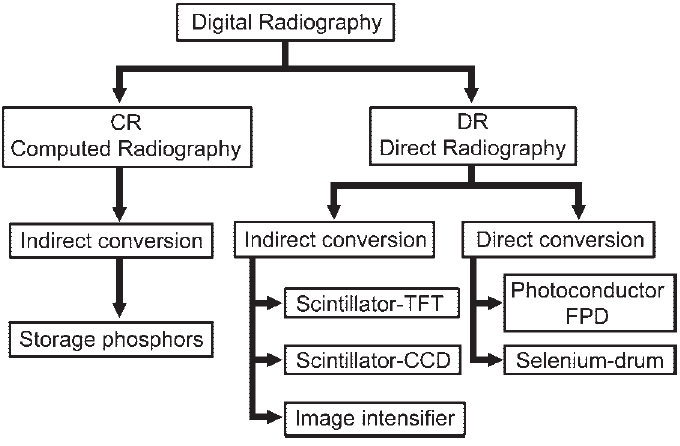
\includegraphics[width=\linewidth]{img/radiohierarchie.png}
  \caption{A systematic overview of various types of digital detectors. CCD =
  chargecoupled device, FPD = flat-panel detector, TFT = thin-film transistor.
  \cite{digitalradio}}
  \label{fig:radiohierarchie}
\end{center}
\end{figure} 

We first discuss the various types in greater detail using
\autoref{fig:radiohierarchie}. The first incarnation of digital radiography -
called computed radiography (CR) - used storage phosphor to temporarily store
the image information, and lasers to read out the values pixel by pixel at a later
stage \cite{digitalradio}. Unfortunately, the physical properties of storage
phosphors severely limited the resolution of the resulting image, reducing their
diagnostic value. The technology underwent many iterations, as shown in
\autoref{tbl:radiotime}.

\begin{table}[ht]
\begin{tabular}{l l}
\hline
Year & Development\\
\hline
1980 & Computed radiography (CR), storage phosphors\\
1987 & Amorphous selenium�based image plates\\
1990 & Charge-coupled device (CCD) slot-scan direct radiography (DR)\\
1994 & Selenium drum DR\\
1995 & Amorphous silicon�cesium iodide (scintillator) flat-panel detector\\
1995 & Selenium-based flat-panel detector\\
1997 & Gadolinium-based (scintillator) flat-panel detector\\
2001 & Gadolinium-based (scintillator) portable flat-panel detector\\
2001 & Dynamic flat-panel detector fluoroscopy�digital subtraction angiography\\
\hline
\end{tabular}
\caption{Timetable of developments in digital radiography \cite{digitalradio}.}
\label{tbl:radiotime}
\end{table}

The alternative to computed radiography is direct radiography (DR). It comes in
two forms, using either direct or indirect conversion. The direct form uses a
photoconductor to convert the incident photons to electrical charges. Typical
semiconductor materials used in photoconductors are amorphous Selenium (a-Se)
and Gadolinium (Gd). In earlier versions the photons were projected onto a
rotating drum and converted to electrical signals using an analog to digital
converter (ADC). Newer versions however use a flat panel detector (FDP) where
the ADC is swapped out for thin-film transistors (TFT, also used in LCD
displays). These TFTs are made of amorphous Silicon (a-Si). Because the used
materials have a very high intrinsic resolution, the final image resolution is
only limited by the quality of the underlying detector array.

\begin{figure}[ht]
\begin{center}
  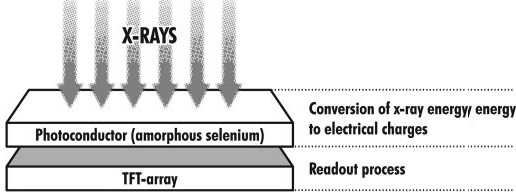
\includegraphics[width=\linewidth]{img/direct_FPD.png}
  \caption{Components of a direct conversion flat panel detector. \cite{digitalradio}}
  \label{fig:directfpd}
\end{center}
\end{figure}

In indirect conversion DR, an extra element is added between the X-rays and the
actual detector. A common example is a scintillator plate that converts X-rays
into visible light. Alternatively, an image intensifier (II) can be used to
amplify the light output. This light can than be captured more easily by a
charge-coupled device (CCD, also used in digital cameras) or a TFT. Because of
the extra step, the point spread function (PSF) increases and the resolution
suffers slightly.

A CCD chip is relatively small so it cannot under normal circumstances record a
whole image at once. Two alternatives are possible. One uses a lens to focus the
rays onto the smaller chip area, but this reduces the image quality. Another
uses a small collimated fan-shaped beam combined with a moving CCD detector.
This system performs comparable to FPDs. One drawback is that this elaborate
setup is not very mobile.

Instead of a CCD, TFTs can also be used in a similar fashion as in direct
conversion DR FPDs. Only this time a scintillator is added. These scintillators
use either Cesium Iodide (CsI) or Gd-based crystals. Contrary to Gd, CsI
crystals can be structured, improving the image quality. The trade-off is their
brittleness, making them less portable. The visible light they emit is then
captured by photo diodes and read out by a TFT array.

\begin{figure}[ht]
\begin{center}
  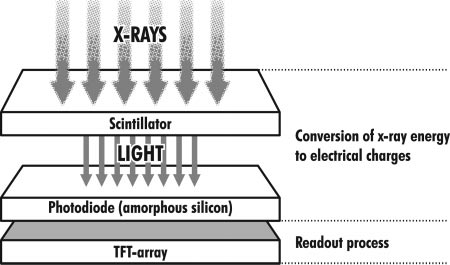
\includegraphics[width=\linewidth]{img/indirect_FPD.png}
  \caption{Components of an indirect conversion flat panel detector. \cite{digitalradio}}
  \label{fig:indirectfpd}
\end{center}
\end{figure}

For the actual assessment, we will focus on both direct and indirect FPDs.

\subsection{Assessing novelty in functionality}
Functionality-wise, we can distinguish between novelty in components and
combinations thereof on the one hand, and novelty in natural effects exploited
on the other hand.

\subsubsection{Novelty in components}
As explained above, digital radiography in general uses many of the same parts
as analogue radiography. Only the detector is fundamentally different. Of course
the real advantage of digitizing radiographs is what you can do with them
afterwards. However, that is out of the scope of this text, and we will
constrain ourselves to the hardware aspects for now.

The next question we ask ourselves is whether these new (combinations) of
components were already used before. The answer is yes. For example CCDs were
invented in 1969 at AT\&T Bell Labs (patents: US3792322,  US3796927) and first
used in digital cameras by 1975 \cite{solidstatesens}. On the other hand, the
combination of a scintillator with CCDs to capture X-rays was not used before. 

In the case of direct FPDs using TFTs, the results are similar. Engineers
experimented with them as early as 1971 for use in display equipment
\cite{lcdhistory}. To this day, they are almost exclusively used in LCD panels
and in digital radiography. In conclusion, they were used before, but mostly in
a field that is not closely related to medical imaging.

\subsubsection{Novelty in natural effects exploited}
Of course the primary natural effect exploited is that of the X-ray passing
through tissue. This has not changed with digital radiography. On the other
hand, the natural effects used in the digital detector are very distinct from
those in classic photographic film. Where such films fall under the
accomplishments of material science, modern digital recording equipment are made
possible by advances in the electronic and semiconductor industry. Obviously
these natural effects were exploited numerous times before by other digital
equipment, but not equipment related to medical imaging.

\subsubsection{Scores}
In \autoref{tbl:funcscores1} we give an overview of the scores on the various topics.

\begin{table}[h]
\centering
\begin{tabular}{l l}
\hline
\multicolumn{2}{|c|}{Novelty in functionality} \\
\hline
A. Novelty of components & B. Novelty in natural effects exploited\\
A1) 4 & B1) 8\\ 
A2) 5 & B2) 5\\ 
\hline
\end{tabular}
\caption{Novelty in functionality scores}
\label{tbl:funcscores1}
\end{table}

\subsection{Assessing novelty in knowledge origins}
Regarding knowledge origins (KOs), we can make a distinction between scientific
and technological origins. To find these KOs, we first provide a list of
problems that had to be solved for digital radiography to become feasible.

The main purpose is to somehow intercept the X-rays and translate their
intensities per pixel into a discrete values that can be processed by a
computer. To do so, they X-rays must first be converted to electrical charges,
which can then be interpreted as bits.

Problem 1: converting the X-ray intensities to bits

Problem 1.1: converting the X-rays to electrical charges

Solution 1.1a: direct conversion: use a photoconducting material (a-Se)

KO1: electromagnetism, semiconductors

Solution 1.1b: indirect conversion: use a scintillator (CsI) and photodiodes (a-Si)

KO2: electromagnetism, material science and semiconductors

Problem 1.2: converting the electrical charges to bits

Solution 1.2: use a TFT array

KO3: digital electronics (mostly transistors)

\subsubsection{Scores}
Electromagnetism falls under scientific origins. The use of electromagnetism
knowledge in medical imaging is certainly nothing special, so it receives low
scores.

The other origins fit better in the technological group. The use of digital
electronics and all related disciplines makes digital radiography what it is.
This warrants a high score, at least for the detector part. However, at
the time of invention the digital electronics industry was booming and
already widely in use in various other fields. In that regard it was only a
matter of time before someone came up with the idea to combine digital
electronics with radiography.

\autoref{tbl:origscores1} shows the scores.

\begin{table}[h]
\centering
\begin{tabular}{l l}
\hline
\multicolumn{2}{|c|}{Novelty in knowledge origins} \\
\hline
A. Novelty of scientific origins & B. Novelty of technological origins\\
A1) 2 & B1) 8\\ 
A2) 2 & B2) 5\\ 
\hline
\end{tabular}
\caption{Novelty in knowledge origins scores}
\label{tbl:origscores1}
\end{table}

\subsection{Assessing technological impact}
The last part of this digital radiography assessments looks into technological
impact. Impact can be split into three parts: performance increase,
technological accumulation and obsoleting previous technologies.

\subsubsection{Performance increase}
The goal of radiography is simply to make clear images that have a high
diagnostic value. To that end, spatial resolution, contrast and noise as
discussed in \autoref{sssec:imgquality} are all important. The aim of digital
resolution was not necessarily to do better in this regard, because analogue
images were already very detailed. If the quality is on par, we should consider
ourselves happy.

As explained above, resolution was a problem with computer radiography using
storage phosphors. However, the materials used in flat panel detectors all have
a high inherent spatial resolution. Only the size of the underlying TFT array
limits the final image resolution. Because analogue radiographs are not
expressed in number of pixels, the performance comparison is complicated.
However, tests performed by \cite{review} show that diagnostic value of analogue
and digital images are almost on par as long as the pixels are about 0.1mm in
size.

Contrast on the other hand is a serious problem for digital radiography. The
deep blacks of photographic film combined with the strong light from a lightbox
creates very high contrast. In comparison, radiologists now have to look at
images on their computer screen in a dark room. On the other hand, digital
radiography makes up for this defect by offering the possibility of
post-processing where it is not only possible to zoom in spatially, but also on
a certain intensity interval (using so-called grey-level transformations
\cite{suetens}). This way, contrast can be increased in one intensity interval
in exchange for lowering it in other intervals.

Noise-wise, the electronic circuits introduce additional electronic noise on top
of the electromagnetic noise. Fortunately, modern electronics can minimize the
former noise, as evident by our crisp digital photographs and big flat screens.

Other advances in performance include: lack of geometric distortion, no veiling
glare, uniform response across the field of view \cite{review}. In addition,
costs are reduces because expensive photographic film is no longer needed, and
time span is reduces because film development happens automatically and almost
instantly.

It is difficult to assign a single score to this component because of the many
issues at play. The image quality did not necessarily improve much, but this was
not the goal. The real performance increase is due to indirect opportunities
opened up by the digital image format. Therefore, in our opinion this still
deserves a fairly high score.

\subsubsection{Technological accumulation}
In this section we estimate the broadness, magnitude and novelty of the impact.

\paragraph{Broadness of impact}
The real breakthrough that made digital radiography possible was the
advent of digital electronics. This breakthrough had a very broad impact on
fields other than its own. Other fields looked directly at digital electronics,
rather than digital radiography, for possible innovations. That is why this
innovation does not score high on broadness of impact. It did however impact
related fields such as CT and PET.

\paragraph{Magnitude of impact}
Although the broadness of impact was not big, and it mostly concentrated on
highly related fields, the magnitude was considerable. In fact, computed
tomography would not even be possible if it were not for the invention of
digital detectors. The same goes (to a lesser extent) for detectors used in
nuclear medicine imaging.

\paragraph{Novelty of impact}
The novelty of impact of digital radiography is very low because other
technologies that never used digital electronics before, got their ideas from
digital electronics in general, not specifically from digital radiography.

\subsubsection{Obsoleting previous technologies}
The last aspect of impact assessment regards obsoleting previous technologies,
i.e.\ analogue radiography. According to \cite{review} and \cite{suetens}, this
has indeed happened. Few radiology departments still stick with analogue systems
because of their lower cost and extreme reliability, but most of the world has
permanently moved on. Not only in radiography, but also in related disciplines
such as CT and PET.

\subsubsection{Scores}
\autoref{tbl:impactscores1} shows the scores.

\begin{table}[h]
\centering
\begin{tabular}{l l l}
\hline
\multicolumn{3}{|c|}{Technological impact} \\
\hline
A. Performance increase & B. Tech. accumulation & Obsoleting previous tech.\\
A) 8 & B1 a) 3 --- b) 1 & C) 10\\ 
     & B2 a) 8 --- b) 7 & \\
     & B3 a) 1 --- b) 1 & \\
\hline
\end{tabular}
\caption{Technological impact scores}
\label{tbl:impactscores1}
\end{table}

\section{CT invention: Electron-beam CT} %US 4352021 A (Boyd, 1982)
Our next assessment deals with an innovation related to computed tomography. In
particular, we take a closer look at Electron-beam Computed Tomography (EBCT),
also know as Ultrafast CT.

\subsection{Defining the technology}
Traditional CT scanners have an X-ray tube embedded in the toroid body. By
mechanically rotating the tube along with the detector, projections from an
arbitrary angle can be captured.

EBCT also needs to be able to capture projections from any angle, but takes
another route. Remember that in a regular X-ray tube current flowing through the
cathode releases electrons. The electrons are accelerated towards the anode by
applying a voltage across the tube. When the electrons hit the anode at high
speed, they release part of their energy as X-rays. The same principle is used
in EBCT, except that the tube is physically split up in two dedicated parts. One
is the cathode or electron gun and is placed along the patient's longitudinal
axis. The other is the anode and is shaped in a semi-ring around the patient.
Using magnetic fields, the electrons fired from the cathode are deflected onto this
ring, where they produce X-rays that can be captured by a detector array as
usual \cite{suetens}. \autoref{fig:ebctscanner} illustrates this.

\begin{figure}[ht]
\begin{center}
  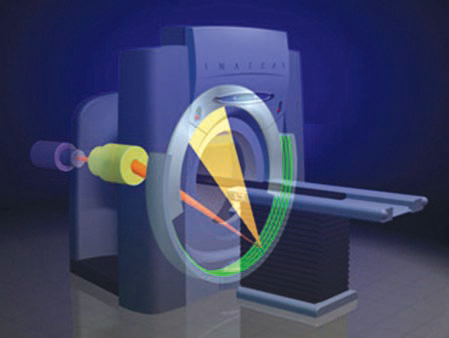
\includegraphics[width=\linewidth]{img/EBCT.png}
  \caption{Rendering of an EBCT scanner's inner workings \cite{suetens}.}
  \label{fig:ebctscanner}
\end{center}
\end{figure}

The main advantage of this setup is that the X-ray source rotation is no longer
mechanical. This allows for faster sweeps, which in turn make it easier to image
moving structures such as the heart. In traditional CT scanners, this movement
would cause blurring in the final image, and thus a loss of diagnostic value.
One very prominent EBCT application is the detection of calcifications from
atherosclerosis in the coronal arteries (i.e., coronary artery disease)
\cite{ultrafastcad}. These are very close to the heart, and can move by about
five times their own diameter every heartbeat.

More recently, these EBCT scanners have received strong competition from
multislice helical CT scanners. The latter enjoy a widespread adoption and are
also less costly (partly due to economies of scale and increased competition).
However, their rotation speed still cannot match that of Ultrafast CT
\cite{ultravshelical}. In addition, this techniques requires a lower dose
compared to traditional CT, and much lower than a CT angiography
\cite{ultralowdose}. The latter is a common alternative for diagnosing coronary
artery disease when an EBCT scanner is not available.

In conclusion, this technique is promising for non-invasive detection of
coronary heart disease, but it has too many unsolved problems to replace general
purpose CT scanners \cite{multictbook}.

\subsection{Assessing novelty in functionality}

\subsubsection{Novelty in components}
As outlined above, the components are largely the same as in conventional CT
scanners. Only their location is different. One additional component is the coil
to generate the deflecting magnetic field. Such electromagnets were used before
in imaging, particularly in MRI, but for a very different purpose.

\subsubsection{Novelty in natural effects exploited}
The same story applies for novelty in natural effects exploited: few new effects
except bending of the electron beam using magnetic fields. The same principle
was used much earlier in Cathode Ray Tube (CRT) monitors and televisions.

\subsubsection{Scores}
In \autoref{tbl:funcscores2} we give an overview of the scores on the various
topics.

\begin{table}[h]
\centering
\begin{tabular}{l l}
\hline
\multicolumn{2}{|c|}{Novelty in functionality} \\
\hline
A. Novelty of components & B. Novelty in natural effects exploited\\
A1) 3 & B1) 3\\ 
A2) 5 & B2) 5\\ 
\hline
\end{tabular}
\caption{Novelty in functionality scores}
\label{tbl:funcscores2}
\end{table}

\subsection{Assessing novelty in knowledge origins}
Again, we look into the problems that had to be solved to find the knowledge
origins. We only look at the problems that are different in comparison to a
traditional CT scanner.

Problem 1: deflect the electron beam onto the anode ring.

Solution 1: use magnetic fields (electric field deflection only works for small angles)

KO1: electromagnetism, CRT monitors

Problem 1.1: overcoming Coulomb repulsion to obtain proper beam focus

Solution 1.1: leak nitrogen into vacuum chamber \cite{ebctelectric}

KO2: charged particle optics

Problem 2: synchronise imaging with heart rhythm

Solution 2: use ECG equipment

KO3: biomedical sensors, signal processing

\subsubsection{Scores}
Electromagnetism, charged particle optics and signal processing can be
considered scientific origins, while the others are technological in nature.

Note that using ECG equipment to synchronise imaging with the heart rhythm is
not new. It was occasionally used before in various other imaging modalities
\cite{suetens}.

\autoref{tbl:origscores2} shows the scores.

\begin{table}[h]
\centering
\begin{tabular}{l l}
\hline
\multicolumn{2}{|c|}{Novelty in knowledge origins} \\
\hline
A. Novelty of scientific origins & B. Novelty of technological origins\\
A1) 4 & B1) 5\\ 
A2) 1 & B2) 1\\ 
\hline
\end{tabular}
\caption{Novelty in knowledge origins scores}
\label{tbl:origscores2}
\end{table}

\subsection{Assessing technological impact}
\subsubsection{Performance increase}
As outlined above, EBCT is very useful for mainly one thing: imaging the heart
and its periphery. However, there are serious drawbacks that do not make it
useful as a general purpose CT scanner. For example, due to the new geometry
X-ray scatter cannot be reduced as effectively. This in turn generates extra
artifacts on the resulting image. The electron gun also has limited power making
it inadequate for higher dosage (i.e., higher contrast) studies \cite{multictbook}.

\subsubsection{Technological accumulation}
Surprisingly, we were unable to identify any newer invention based on EBCT.
Various other applications using electron beams were checked, such as electron
microscopes and electron beam lithography, but none seem to be based on
innovations in EBCT. This may be caused by the relative obscurity of EBCT
outside of medical imaging fields.

\subsubsection{Obsoleting previous technologies}
EBCT has definitely not obsoleted previous technologies. Its application area is
simply too narrow for many hospitals to warrant such an expensive purchase.
Instead, older and cheaper but less effective methods are still used more often
to diagnose coronary artery disease. Examples include a CT angiography, exercise
stress tests but also invasive (catheter) examinations.

\subsubsection{Scores}
\autoref{tbl:impactscores2} shows the scores.
\begin{table}[h]
\centering
\begin{tabular}{l l l}
\hline
\multicolumn{3}{|c|}{Technological impact} \\
\hline
A. Performance increase & B. Tech. accumulation & Obsoleting previous tech.\\
A) 5 & B) N/A & C) 2\\ 
\hline
\end{tabular}
\caption{Technological impact scores}
\label{tbl:impactscores2}
\end{table}

\section{MRI invention}
Normally we only consider inventions from 1980 onwards, but for this section we
would like to make an exception. The invention of the MRI scanner itself was a
veritable breakthrough, and still happened relatively close to 1980. Because we
already had a close look at MRI in \autoref{sec:mri}, we will skip the
technology definition and go straight to the assessment.

\subsection{Assessing novelty in functionality}
\subsubsection{Novelty in components}
The purpose of MRI scanners is largely the same as that of CT scanners: create
cross-sectional images to look into patient's bodies without using invasive
techniques. The essential components of CT are the X-ray source and the
detector. With MRI, we again have a signal source and a signal detector.
However, this time the source is a large electromagnet, and the detector is a
quadrature detector.

Electromagnets are used in various other technologies to do the same thing:
generate magnetic fields. Examples include motors, generators, transformers,
relays and loudspeakers. In that sense the choice was not very special.

Similarly, quadrature detectors are used universally whenever signal
demodulation is required \cite{quadrature}. Remember that MRI operates in the
radio frequency range, so ordinary radio technology could be repurposed for use
in these scanners.

In summary, these components were not used in medical imaging before the advent
of MRI. Yet, once it was decided to exploit radio waves and magnetic fields, the
choice of components was rather trivial.

\subsubsection{Novelty in natural effects exploited}
MRI has one thing in common with the other imaging modalities discussed: they
all use electromagnetic radiation in one form or another. Nevertheless, the way
this natural effect is exploited here is considerably different from other
modalities. In radiography and CT, we measure the X-ray attenuation when
traveling through the human body. With nuclear medicine, we essentially detect
photons emitted by radioactive materials. MRI on the other hand influences and
measures the magnetic properties of tissues, in particular the proton density,
the $T_1$ time or the $T_2$ time.

In a way, every researcher that ever worked on imaging based on magnetic fields
contributed to the eventual creating of MRI. Of course some groups took a
slightly different turn (e.g. measuring properties of electrons instead of
protons), but their larger goal was the same. To our knowledge no one
experimented with these specific magnetic properties for any other purposes.

\subsubsection{Scores}
In \autoref{tbl:funcscores3} we give an overview of the scores on the various
topics.

\begin{table}[h]
\centering
\begin{tabular}{l l}
\hline
\multicolumn{2}{|c|}{Novelty in functionality} \\
\hline
A. Novelty of components & B. Novelty in natural effects exploited\\
A1) 10 & B1) 8\\ 
A2) 3 & B2) 8\\ 
\hline
\end{tabular}
\caption{Novelty in functionality scores}
\label{tbl:funcscores3}
\end{table}

\subsection{Assessing novelty in knowledge origins}
Once again, we start with a list of problems and corresponding solutions.

Problem 1: measure proton density in tissue

Problem 1.1: align net magnetization vectors

Solution 1.1: generate a large magnetic field

KO1: electromagnetism

Problem 1.1.1: increase field strength, lower power consumption

Solution 1.1.1: superconductivity by extreme cooling

KO2: physics (cryogenics), material science

Problem 1.2: measure magnetization vector

Solution 1.2a: disturb equilibrium with the appropriate pulse sequence

KO3: theory from electromagnetism, but to our knowledge never exploited before

Solution 1.2b: record relaxation phenomena using quadrature detector

KO4: analogue electronics, radio equipment 

Problem 2: localize position using signal

Solution 2: apply a magnetic field gradient

KO5: electromagnetism, gradients recently used in \cite{nanogradients1,
nanogradients2}, older: \cite{oldgradients}.

\subsubsection{Scores}
None of these knowledge origins, except the usage of specific pulses, is out of
the ordinary. Radio equipment is also a new technological origin, but its
purpose in other inventions is very similar. That is why in
\autoref{tbl:origscores3} we give low scores except for this technological
origin.

\begin{table}[h]
\centering
\begin{tabular}{l l}
\hline
\multicolumn{2}{|c|}{Novelty in knowledge origins} \\
\hline
A. Novelty of scientific origins & B. Novelty of technological origins\\
A1) 2 & B1) 6\\ 
A2) 2 & B2) 7\\ 
\hline
\end{tabular}
\caption{Novelty in knowledge origins scores}
\label{tbl:origscores3}
\end{table}

\subsection{Assessing technological impact}
\subsubsection{Performance increase}
Although we have portrayed MRI as the successor to CT in the section above, this
is not completely true. MRI allows us to visualize things we could not before
with CT. For example, cancerous tissue is sometimes easier to spot on MRI scans.
Whereas on CT scans the attenuation properties of both tissue types might be
very similar, malignant tumors appear to exhibit a larger $T_1$ value than
surrounding tissue \cite{mrihistory}.

On the other hand, CT has the advantage when it comes to visualizing bone.
Because it contains few free hydrogen atoms, it is very difficult to spot on an
MRI scan. X-rays however are ideal for this type of diagnosis.

In conclusion, it is very difficult to unilaterally award the performance
trophy to either side. 

\subsubsection{Technological accumulation}
\paragraph{Broadness of impact}
MRI generated a lot of spin-off technologies, including Magnetic Resonance
Angiography (MRA), Magnetic Resonance Spectroscopy (MRS) and functional MRI
(fMRI). These are of course all part of the same imaging family, and we could
not find any impact outside of this family in the literature. Perhaps
mining through patents can show some interesting results. 

\paragraph{Magnitude of impact}
Although the broadness is limited, the magnitude of impact is substantial.
Especially for the direct spin-offs listed above, but also indirectly through
the spin-offs of those spin-offs.

\paragraph{Novelty of impact}
As stated above, we only identified direct impact on its immediate spin-off
technologies. The degree of novelty is thus very low.

\subsubsection{Obsoleting previous technologies}
As stated before in \autoref{ssec:mrifuture}, MRI has not replaced CT, but is
expected to gain more traction in the future. For now, the two technologies are
complimentary: each is better for a specific subcategory of diagnostic imaging. 

\subsubsection{Scores}
\autoref{tbl:impactscores3} shows the final scores.

\begin{table}[h]
\centering
\begin{tabular}{l l l}
\hline
\multicolumn{3}{|c|}{Technological impact} \\
\hline
A. Performance increase & B. Tech. accumulation & Obsoleting previous tech.\\
A) 5 & B1 a) 4 --- b) 2 & C) 3\\ 
     & B2 a) 8 --- b) 8 & \\
     & B3 a) 1 --- b) 1 & \\
\hline
\end{tabular}
\caption{Technological impact scores}
\label{tbl:impactscores3}
\end{table}

\section{Nuclear medicine invention: 18F-FDG tracers}
In this assessment related to nuclear medicine we focus on something slightly
unusual. Not a component or new technique used in the scanner, but on one of the
popular tracers used during such examinations: $^{18}$F-FDG tracers.

\subsection{Defining the technology}
PET scanners work by detecting positrons formed by the decay of radioactive
tracers, as explained in \autoref{chap:nuclearimg}. The most commonly used
isotope is fluorine-18. It is very suited for PET because it almost exclusively
emits positrons when decaying to oxygen-18. Its half life of 110 minutes gives
it another attractive property.

%The first incarnation of these kind of glucose-based tracers was 

However, the fluorine isotope is only responsible for the emission of positrons,
it cannot be absorbed by or transported in the human body on its own. That is
where 2-deoxy-2-fluoro-D-glucose or, more conveniently fluorodeoxyglucose (FDG),
comes into play. One of its hydroxyl (-OH) groups can be replaced by
fluorine-18. Because it is analogous to normal glucose, its uptake in the body
is also similar. However, unlike normal glucose it cannot be completely
metabolised as long as the fluorine isotope is present. Instead, it gets stuck
in the cells until the fluorine decays into oxygen and it can form a hydroxyl
group again.

When the tracer is injected into the body, a PET scanner can visualize its
distribution throughout the various tissues. This way, physicians can monitor
glucose metabolism and spot abnormalities or deviations. Those can be caused by
tumors for example, which typically grow very fast and consequently need lots of
energy. Brain activity can also be measured regionally because active parts of
the brain tend to metabolise more glucose.

Synthesis of FDG is possible in a number of ways, but most are rather
sophisticated. 

%impact: neuroscience, oncology

%1948: NO, Fick principle, cerebral bloodflow (global)
%1977: Sokoloff, C14-glucose [20]
%1979: Reivich [21], FDG, Ido et al. [22]
%uses: table 1

\subsection{Assessing novelty in functionality}

\subsubsection{Novelty in components}
The F-FDG tracer is a composite made out of both FDG and fluorine-18. Earlier
tracers also used FDG, but the isotopes were different. Carbon-14 was a popular
choice \cite{radiopharma}. The fluorine-18 seems to be exclusively used as a
radioactive tracer. It is sometimes also combined with other molecules, for
example to track dopamine instead of glucose \cite{fluorodopa, fdopamine}.
Another isotope (fluorine-19) is used as a contrast agent in MRI studies.

The first paper describing the synthesis of F-FDG already mentioned specific
usage as a radiopharmaceutical \cite{firstF-FDG}. To our knowledge, it has not
been used outside this context. Within this context however, it was used towards
many different goals in biomedical research such as neuroscience and oncology. 

\subsubsection{Novelty in natural effects exploited}
The tracer isotope exploits radioactive decay, more specifically positron
emission decay. Considering PET works exclusively with positron emission decay,
this is no special feat. However, what makes fluorine-18 special is that it
hardly has any other decay mechanisms and that its half life has the ideal
length for PET studies.

The second natural effect exploited is how the human body treats FDG very
similar to normal glucose.

\subsubsection{Scores}
In \autoref{tbl:funcscores4} we give an overview of the scores on the various
topics.

\begin{table}[h]
\centering
\begin{tabular}{l l}
\hline
\multicolumn{2}{|c|}{Novelty in functionality} \\
\hline
A. Novelty of components & B. Novelty in natural effects exploited\\
A1) 6 & B1) 3\\ 
A2) 2 & B2) 1\\ 
\hline
\end{tabular}
\caption{Novelty in functionality scores}
\label{tbl:funcscores4}
\end{table}

\subsection{Assessing novelty in knowledge origins}
To make F-FDG work, a number of problems had to be overcome.

Problem 1: find a tracer that emits positrons

Solution 1: the following isotopes are known to emit positrons:  carbon-11,
nitrogen-13, oxygen-15, fluorine-18, sodium-22, aluminium-26, potassium-40, 
and iodine-121

KO1: nuclear physics

Problem 1.1: find an isotope that easily combines with lots of molecules 

Solution 1.1: carbon-11 and fluorine-18 \cite{radiopharma}

KO2: biochemistry

Problem 1.2 find an isotope that has a suitable half life for PET studies

Solution 1.2 fluorine-18

KO3: nuclear physics

Problem 2: find a suitable transport molecule that mimics glucose

Solution 2: replace one hydroxyl group in normal glucose with an isotope 

KO4: biochemistry, pharmacology

\subsubsection{Scores}
\autoref{tbl:origscores4} shows the scores. Note that there are no technical
knowledge origins. This is a consequence from the rather unique category of
innovation radiopharmaceuticals belong to. The scientific knowledge origins on
the other hand are rather straightforward for these kinds of applications.

\begin{table}[h]
\centering
\begin{tabular}{l l}
\hline
\multicolumn{2}{|c|}{Novelty in knowledge origins} \\
\hline
A. Novelty of scientific origins & B. Novelty of technological origins\\
A1) 1 & B1) N/A\\ 
A2) 1 & B2) N/A\\ 
\hline
\end{tabular}
\caption{Novelty in knowledge origins scores}
\label{tbl:origscores4}
\end{table}

\subsection{Assessing technological impact}
\subsubsection{Performance increase}
Performance of positron emission tracers is difficult to quantify. Remember that
in nuclear medicine the image quality is of secondary importance. More important
is the fidelity of the tracer. It should properly visualize the biochemical and
physiological processes, glucose metabolism in our case. Empirical tests
confirmed that FDG is effectively processed in the same manner as normal glucose
in the body, and that PET scans highlight regions where glucose metabolism is
expected to be higher (brains, kidneys, tumors) \cite{radiopharma}. Earlier
incarnations such as $^{11}$C-glucose also achieved this. Unfortunately, because
of the short half life of just 20 minutes, images had to be taken before the
tracer had the chance to diffuse properly.

\subsubsection{Technological accumulation}
\paragraph{Broadness of impact}
The success of F-FDG inspired the production of several other tracers. One
example is a tracer called F-fluoro-DOPA for studying dopamine utilization
\cite{radiopharma}.

However, the biggest impact by far was on research in the fields of medicine and
physiology. This tracer opened up lots of new possibilities, and application in
oncology, neuroscience, virology etc. \cite{fdgresearch1, fdgresearch2}.

\paragraph{Magnitude of impact}
As stated before, the invention of FDG led to many spin-off tracers, and each of
those tracers has multiple spin-offs itself. The magnitude of impact is thus
significant.

\paragraph{Novelty of impact}
Fields such as virology could traditionally not make use of imaging modalities,
because viruses are simply too small to be seen. However, FDG-related
technologies in combination with PET scanners have allowed researchers to
finally see what exactly goes on at this microscopic level \cite{fdgresearch2}.

On the other hand, most of the impact was on fields that already made extensive
use of imaging modalities, such as oncology or neuroscience.

\subsubsection{Obsoleting previous technologies}
These days PET and F-FDG are so intricately linked that it is hard to imagine a
time before this tracer was used. Yet, research in this field is still ongoing
and very active. Other biochemical processes obviously require different
transport molecules, and not all of them are compatible with fluorine-18. That
is why many other tracers are still in use today. But when it comes to
visualizing glucose metabolism, F-FDG seems to be the gold standard for now
\cite{radiopharma}.

\subsubsection{Scores}
\autoref{tbl:impactscores4} shows the scores.

\begin{table}[h]
\centering
\begin{tabular}{l l l}
\hline
\multicolumn{3}{|c|}{Technological impact} \\
\hline
A. Performance increase & B. Tech. accumulation & Obsoleting previous tech.\\
A) 7 & B1 a) 7 --- b) 3 & C) 8\\ 
     & B2 a) 7 --- b) 6 & \\
     & B3 a) 4 --- b) 3 & \\
\hline
\end{tabular}
\caption{Technological impact scores}
\label{tbl:impactscores4}
\end{table}

\section{CAD invention: machine learning techniques for mammography}
For this last assessment, we draw from the field of Computer-aided Detection and
Diagnosis. For the rest of this section, we will focus on the usage of machine
learning techniques for CADe in mammography. Breast cancer is one of the
deadliest cancers among women today, but fortunately early detection
significantly improves the chances of survival \cite{mammoairecent}. To detect
breast cancer, phycisians look for calcifications, masses and architectural
distortions on high resolution radiographs (mammograms). Traditionally, every
image is checked by at least two radiologists to increase sensitivity. This is
known as the second reader principle. However, this approach effectively doubles
the workload of the radiology department. Perhaps more than in any other
medical field, CAD can help radiologists by acting as a surrogate second reader
for mammograms. \cite{mlinmedical}.

One particular application where CAD has proven its worth, is in the detection
of microcalcifications in mammograms. These are small calcium deposits of 0.05mm
to 1mm in size that appear as bright white spots on the scan. They are known to
appear in 30-50\% of all breast cancer cases, and are thus an important
indicator. Due to their variable shape, brightness and size, they can be
difficult to detect in the surrounding tissue \cite{mlinmedical}.

Note that - unlike tangible inventions - software algorithms are not so
straightforward to assess using the radical innovation framework. For example,
algorithms typically do not exploit natural effects directly (but computers do).
However, we will make an effort to make a meaningful assessment regardless.

%\cite{mammoai}

\subsection{Defining the technology}
As explained in \autoref{ssec:cadadv}, machine learning comprises a large group
of methods and techniques. We are specifically interested in (binary)
classifiers to determine whether a particular structure on a mammogram is
suspicious enough. The exact nature of this classifier - whether it is a Support
Vector Machine (SVM) or Random Forests (RF) or anything else - is of little
interest for this assessment. We will simply look at them as one group with one
goal.

When assessing this technology, we will compare it to earlier incarnations of
CAD software without machine learning elements, and - where appropriate - with
manual diagnosis by a physician.

\subsection{Assessing novelty in functionality}
Because we are dealing with software algorithms, we can only assess the novel
functionality based on novelty in components, not on novelty in natural effects
exploited. 

\subsubsection{Novelty in components}
In \autoref{ssec:cadtech}, we discussed the generic scheme that most CAD systems
follow. Each of these steps can be considered a separate component in the
algorithm. In our case, step III and IV are replaced by machine learning
algorithms.

Of course these algorithms were used before in a variety of other applications,
but not necessarily related to diagnostic medical imaging
\cite{machinelearningapps}. 

\subsubsection{Scores}
In \autoref{tbl:funcscores5} we give an overview of the scores on the various
topics.

\begin{table}[h]
\centering
\begin{tabular}{l l}
\hline
\multicolumn{2}{|c|}{Novelty in functionality} \\
\hline
A. Novelty of components & B. Novelty in natural effects exploited\\
A1) 5 & B1) N/A\\ 
A2) 4 & B2) N/A\\ 
\hline
\end{tabular}
\caption{Novelty in functionality scores}
\label{tbl:funcscores5}
\end{table}

\subsection{Assessing novelty in knowledge origins}
As usual, we start by listing problems encountered during development of this
invention, and present the proposed solution and its related knowledge origin.
We again follow the five step detection scheme introduced before. 

Problem 1: detect abnormalities in mammograms

Problem 1.1: segment the region of interest

Solution 1.1: trivial, the mammogram only contains the region of interest

Problem 1.2: enhance abnormalities

Solution 1.2: use traditional image processing and computer vision methods
(e.g.\ convolution filters)

KO1: image processing

Problem 1.3: detect and segment abnormalities

Problem 1.3.1: detect abnormalities

Solution 1.3.1: use an appropriately trained machine learning classifier

KO2: statistics, artificial intelligence, machine learning

Problem 1.3.2: segment abnormalities

Solution 1.3.2: use traditional image processing and computer vision methods
(e.g.\ region growing)

KO3: image processing

Problem 1.4: perform feature analysis and classification

Solution 1.4: use an appropriately trained machine learning classifier

KO4: statistics, artificial intelligence, machine learning

Problem 1.5: reduce false positives

Solution 1.5: use traditional false positive reduction methods

KO5: statistics, machine learning

\subsubsection{Scores}
Of the listed knowledge origins, we classify statistics as scientific, and
the rest as technological.

Statistics forms the fundamental basis for almost all machine learning
algorithms. Some more primitive image processing techniques also explicitly use
statistical theory, but most do not. The radiologists that perform a manual
diagnosis use their advanced human visual system instead of relying on
statistics.

Of the technological knowledge origins, machine learning is by definition the
only new element compared to earlier methods.

\begin{table}[h]
\centering
\begin{tabular}{l l}
\hline
\multicolumn{2}{|c|}{Novelty in knowledge origins} \\
\hline
A. Novelty of scientific origins & B. Novelty of technological origins\\
A1) 6 & B1) 3\\ 
A2) 1 & B2) 5\\ 
\hline
\end{tabular}
\caption{Novelty in knowledge origins scores}
\label{tbl:origscores5}
\end{table}

\subsection{Assessing technological impact}
\subsubsection{Performance increase}
Already in 1990, \cite{cadsynergy} proved using observer studies that
radiologists' performance in detecting microcalcifications could increase when
using CAD systems, even if the number of false positives at the time were still
fairly high. The review article \cite{cadhistory} looked into various large
scale studies regarding CAD in mammography, and found that all of them reported
an increase in detection performance compared to pre-CAD diagnosis. Remember
that performance is this context is the combined performance of physician plus
computer, not computer alone. It should be mentioned that other studies found no
performance gain, or even a performance decrease \cite{mammocadbad}, but they
seem to be in the minority. They particularly lament the high number of false
positives, claiming that these cause more unnecessary examinations and
consequently an increase in medical insurance expenditures.

\subsubsection{Technological accumulation}
false positive reduction
\paragraph{Broadness of impact}
Machine learning is generally application-agnostic and thus a very versatile
technique used in a variety of fields, from the financial world over social
networks to medical applications. In fact, CAD was fairly late to jump on the
machine learning bandwagon \cite{mlinmedical}. Nonetheless, a lot of related
research is performed by biomedical scientists. This research is often generic
enough in nature to potentially be applied to other fields again. Unfortunately,
researchers outside of the medical field tend to ignore medical journals in
favor of their own field-specific alternatives. This severely degrades the
possible cross-pollination across fields, and in turn the broadness of impact.
This is evident by the lack of medical literature citations from outside the
field.

\paragraph{Magnitude of impact}
Globally speaking, the medical field only accounts for a relatively small slice
of all machine learning research. Consequently, most breakthroughs will
originate elsewhere, negatively impacting the magnitude of direct and
indirect impact of CAD on unrelated applications.

\paragraph{Novelty of impact}
Due to the versatility of machine learning, there is a lot of potential
for novelty of impact. But again, because of invisible walls surrounding the
medical field, we could not locate specific applications that drew from
biomedical machine learning research.

\subsubsection{Obsoleting previous technologies}
Within three years of FDA approval, about 10\% of of U.S. facilities switched to
CAD technology\footnote{\url{http://www.nih.gov/news/pr/apr2007/nci-04b.htm}}.
CAD technology using machine learning has not yet obsoleted conventional
mammography diagnosis, although performance definitely increases when employed.
Some physicians are simply reluctant to rely on technology for performing their
diagnosis. This will require a change in mindset, which is a long-term endeavor.
On top of that, these systems imply an additional cost on top of the already
expensive imaging equipment. Perhaps integrating them as modules in PACS as
suggested by \cite{cadhistory} will speed up their adoption. Because of these
reasons, researchers believe it is only a matter of time before such methods are
used globally.

\subsubsection{Scores}
\autoref{tbl:impactscores5} shows the scores.

\begin{table}[h]
\centering
\begin{tabular}{l l l}
\hline
\multicolumn{3}{|c|}{Technological impact} \\
\hline
A. Performance increase & B. Tech. accumulation & Obsoleting previous tech.\\
A) 7 & B1 a) 3 --- b) 5 & C) 4\\ 
     & B2 a) 3 --- b) 2 & \\
     & B3 a) 3 --- b) 2 & \\
\hline
\end{tabular}
\caption{Technological impact scores}
\label{tbl:impactscores5}
\end{table}

\section{Conclusion}
In this chapter, we presented the results of the assessment of various
innovations related to diagnostic medical imaging. We tried to be as varied as
possible in the selection of innovations. Not only did they all stem from a
different field, but their scope and type also varied. For example, we tried a
high-level assessment of MRI as a whole, but also assessment of a whole class of
algorithms and a very specific radiopharmaceutical compound. In our newfound
experience, the assessment framework seems to work best on rather low-level, yet
tangible innovations. Nonetheless, it showed considerable flexibility when
applied to concepts it was perhaps never intended for.

Truthfully, we are slightly disappointed by the seemingly low scores of these
important innovations. We explore some reasons for this in the following
paragraphs.

We have tried to make this assessment as detailed as possible. However, medical
imaging is a very complex matter, and even our introduction in
\autoref{chap:imaging} - much like many a review paper - just barely scratch the
surface of all underlying methods and technologies. These details only become
apparent when hands-on work is performed by scientists and researchers in the
field. For example, a little known fact is that the anode in an X-ray tube gets
hot during operation, lowering performance. A simple solution is to make it spin
to cool it down. Such details will only be described in the most detailed
literature and of course in patent applications. We fear that this discrepancy
in level of detail will significantly hamper comparison with the automated
patent analysis.

The way the framework is built also seems to favor automatic patent based
analysis over manual assessment. The questions on the assessment sheet map
nicely to data that can be extracted from patents. On the other hand, manually
finding an answer to these questions without looking at patent data has proven
to be challenging at times. The granularity of the scores presents another
problem. It is very difficult to explain the difference between, say, a 5 and a
6. In that regard we would propose a rescaled score chart with scores from 1 to
5. The alternative is to improve the existing score chart with a more detailed
description of how to quantify the small differences in score.

In addition, the 1980 limit made it significantly more difficult to go back to
the real breakthrough invention, the so-called seed. For example, FDG in nuclear
medicine was certainly a breakthrough but it would have been more interesting to
go back further and see who first managed to bring nuclear physics together with
biochemistry and truly invent radiopharmacology. The fact that many
imaging-related inventions spend a very long time in the research phase, taking
decades before entering the market, does not help in this regard either. On the
other hand, due to the ex-post nature of some assessment questions (i.e.,
impact), very recent innovations cannot be mapped either.

One final aspect we noticed, is that medical imaging research seems to ``stay in
the family'' - so to speak. One imaging modality builds on top of another
modality's body of knowledge, but the technology hardly seems to diffuse into
other fields. One possible explanation is that biomedical researchers have plenty of
very specific medicine-related journals to choose from for publishing, so they
don't branch out. They do not interact much with journals that have similar
content but focus on another sector. From personal experience, this is very
apparent in the image processing literature. For example, one can browse image
processing journals from IEEE in vain trying to find a solution for a generic
non-medical problem. Meanwhile, medical researchers might have come up with such
a solution years ago, applied it to medicine and published it in a medical image
processing journal. Clearly, many disciplines could learn from research in the
biomedical sector.


\chapter{Conclusion}\label{chap:conclusions}
The centerpiece of this thesis is radical innovation. Such innovations have
regularly been seen in the past, and seem to be a key factor in the long term
growth of firms or even entire regions. It follows that identifying such radical
innovations early is critical. Chapter \ref{chap:intro} introduced the reader to
a framework based on three dimensions that does just this. These three
dimensions are novelty in knowledge origins, novelty in functionality
and technological impact. Innovations that score high on all three components
are very likely to be radical. In addition, the framework proposes patent
indicators to automatically score innovations using complex computer algorithms.

In this text however, we restricted ourselves to a thorough manual assessment of
a few innovations in the field of diagnostic medical imaging. To that end, we
presented a short introduction to this field in \autoref{chap:imaging}. In
particular, we discussed the history, technical background, recent advancements
and future expectations of four imaging modalities: radiography, computer
tomography, magnetic resonance imaging and nuclear medicine imaging. We also
briefly discussed computer aided detection and diagnosis.

Once we had a basic understanding of the field, \autoref{chap:inventions}
provided us with a deeper understanding of some more recent innovations in the
field. For each innovation, scores were given based on the assessment sheet in
the appendix. These innovations include digital radiography, electron beam
computed tomography, magnetic resonance imaging, fluorodeoxyglucose tracers and
modern computer aided detection and diagnosis techniques. The scores turned out
lower than expected, and we listed a few possible reasons for this.

This work can serve as a basis to validate and further refine the radical
innovation framework. By comparing the results of this manual assessment with
the outcome of an automatic assessment based on patent indicators, potential
discrepancies and flaws in the framework can hopefully be found and alleviated.

\clearpage %clearbothpages?
\bibliographystyle{alpha} %plain,unsrt,alpha,abbrv,acm,apalike,siam,ieeetr,..
\bibliography{references} \addcontentsline{toc}{chapter}{Bibliografie}

%\vfill

\appendix
\begin{landscape}
	\chapter{Assessment sheet}\label{app:score}
	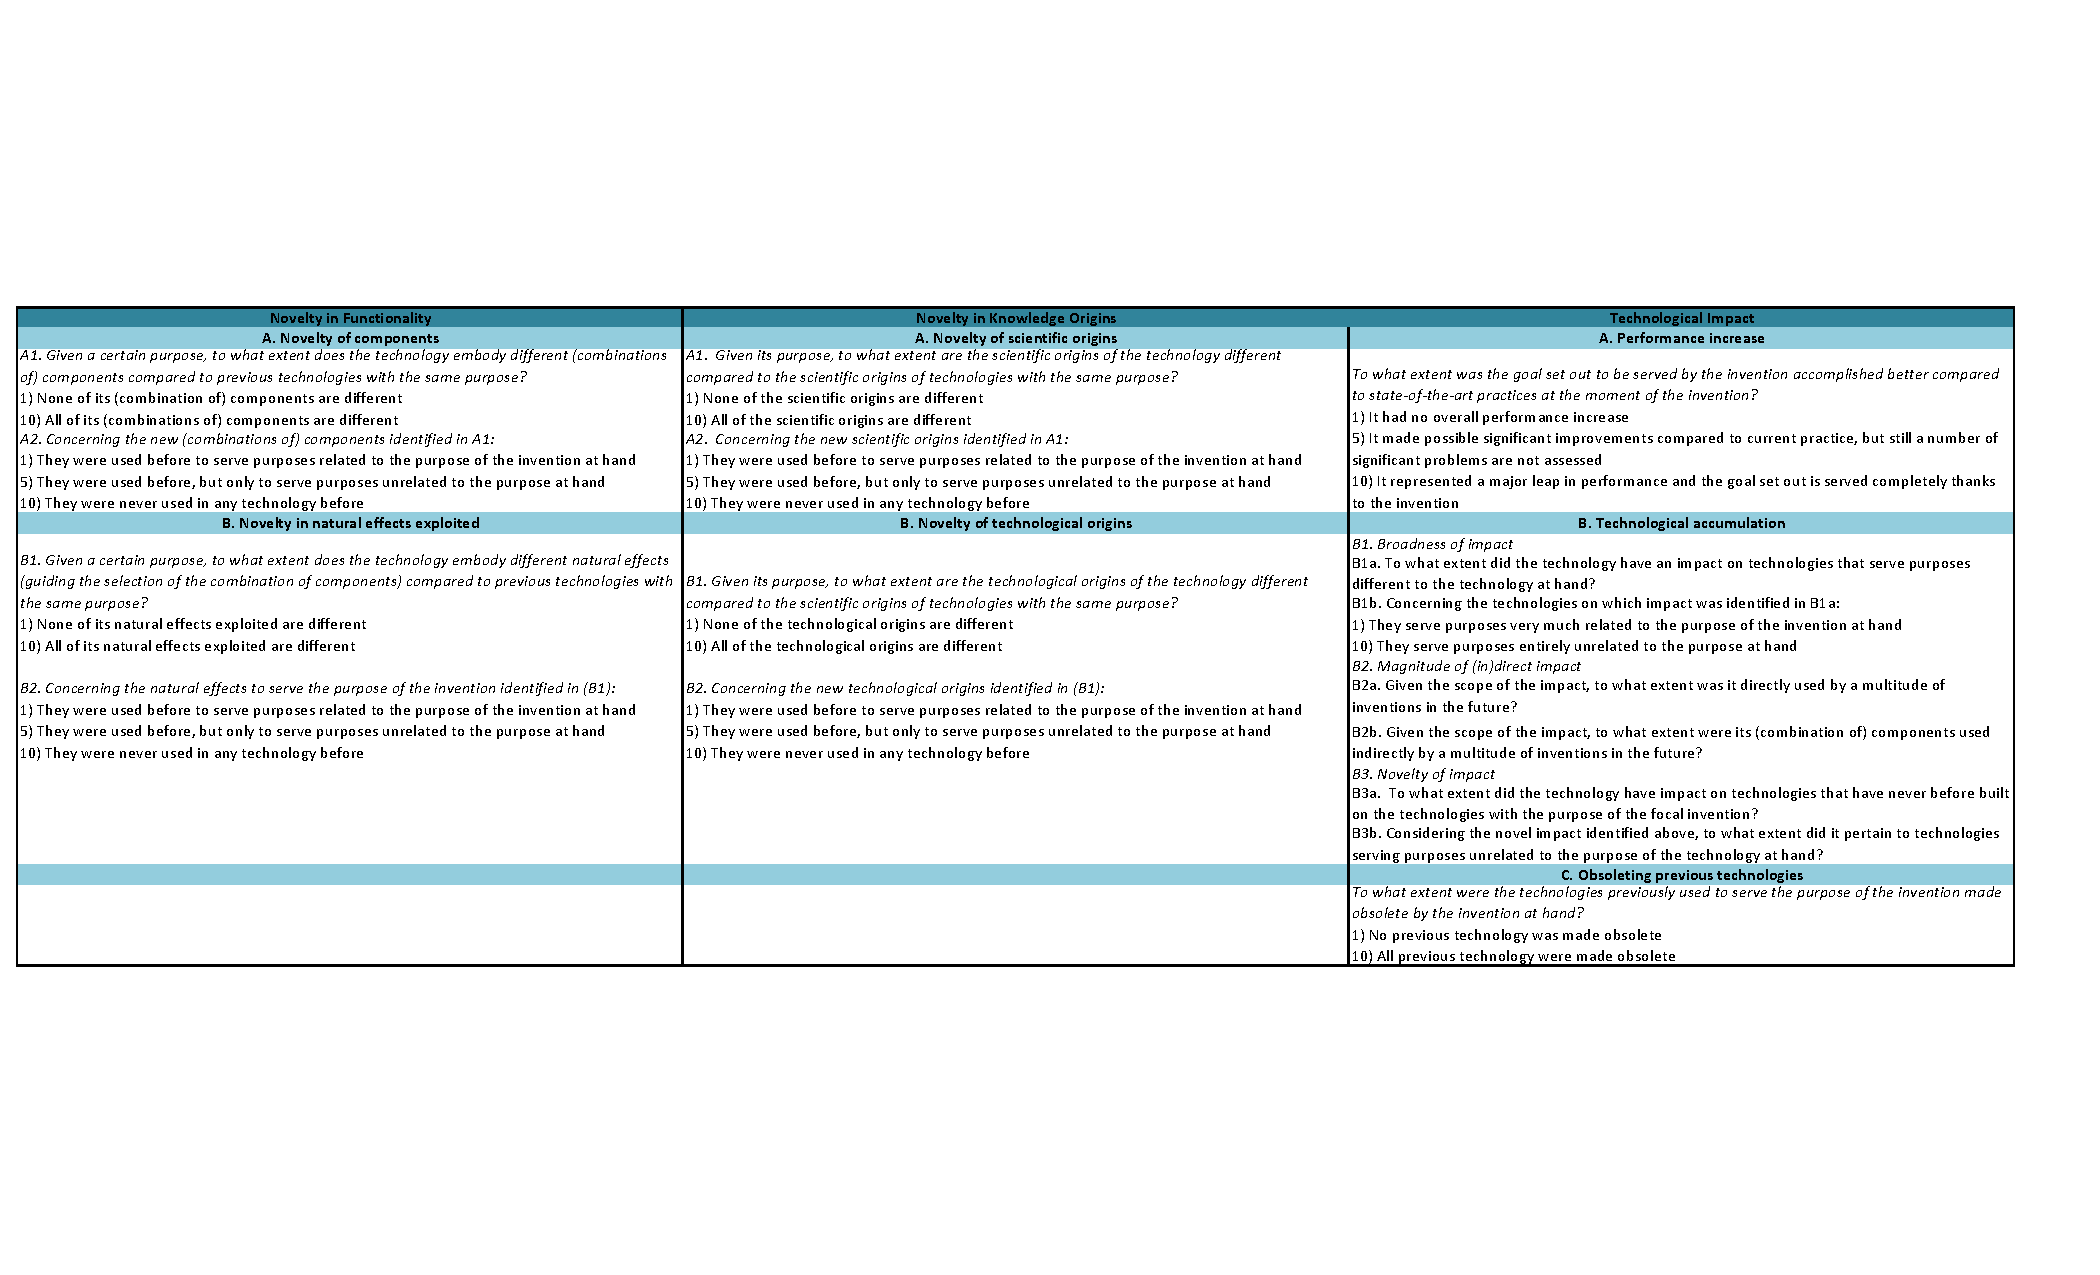
\includegraphics[width=1.0\linewidth, trim=5 150 60 150]{img/score.pdf}
\end{landscape}

\chapter{International Patent Classification codes}
This section contains a list of relevant patent categories in relation to
diagnostic medical imaging. The categories are identified using their
International Patent Classification (IPC) codes. A complete reference of all IPC
codes can be found at \url{http://web2.wipo.int/ipcpub}.

\begin{description}
  \item[A61B 1/005] Flexible endoscopes
  \item[A61B 5/05] Measuring for diagnosis by means of electric currents or magnetic fields
  \item[A61B 6/00] Apparatus for radiation diagnosis, e.g. combined with radiation therapy equipment
  \item[A61B 6/03] Computerised tomographs
  \item[A61B 8/00] Diagnosis using ultrasonic, sonic or infrasonic waves
  \item[G01N 23/00] Investigating or analysing materials by the use of wave or particle radiation
  \item[G01R 33/00] Arrangements or instruments for measuring magnetic variables
  \item[G01T 1/36] Measuring spectral distribution of X-rays or of nuclear radiation
  \item[G01T 1/161] Applications in the field of nuclear medicine, e.g. in vivo counting
  \item[G02B 23/24] Instruments for viewing the inside of hollow bodies, e.g. fibrescopes
  \item[G03B 42/02] using X-rays
  \item[G06T] IMAGE DATA PROCESSING OR GENERATION, IN GENERAL 
  \item[H01J 35/00] X-ray tubes
  \item[H05G] X-RAY TECHNIQUE
\end{description}

\newpage
\thispagestyle{empty}
\newgeometry{textwidth=540pt,textheight=780pt,top=20pt,left=20pt,right=20pt}
\begin{figure}[ht]
\begin{flushright}
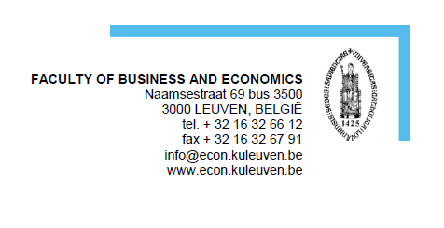
\includegraphics[width=0.5\textwidth,natwidth=310,natheight=10]{img/Picture3.png}	
\end{flushright}
\end{figure}
\vfill
\begin{picture}(550,40)
\put(0,0){\colorbox{kuleuven}{\makebox(520,52){}}}
\end{picture}
\end{document}